\documentclass[14pt]{book}
\usepackage[p,osf]{scholax}
\usepackage{amsfonts,amstext,amsbsy,amsopn,amsmath,eucal,bm,mathrsfs}
\usepackage[T1]{fontenc}
\usepackage{tgbonum}
\usepackage[scaled=1.075,ncf,vvarbb]{newtxmath}% need to scale up math package 
\normalfont
\usepackage[parfill]{parskip}% Begin paragraphs with an empty line rather than an indent

\usepackage{setspace,lineno,enumitem,fancyhdr,marginnote,hyperref}
\usepackage[capitalise]{cleveref}
\usepackage{pstool,pgfplots}
\usepackage[centering,text={18cm,22cm},showframe=false]{geometry}
\pagestyle{fancy}

\usepackage{wrapfig,graphicx,color,xcolor}
\usepackage[labelformat=empty]{caption}
\usepackage{multicol}
\usepackage{multirow}
\usepackage{booktabs}
\definecolor{light-gray}{gray}{0.96}
\definecolor{light-red}{rgb}{0.82, 0.1, 0.26}
\definecolor{light-smoke}{rgb}{0.96,0.96,0.93} 
\definecolor{light-olive}{rgb}{0.63,0.57,0.33} 
\definecolor{light-azul}{rgb}{0.25, 0.41, 0.88}
\definecolor{light-red}{rgb}{0.82, 0.1, 0.26}
\newcommand{\gc}[1]{\textcolor{light-azul}{#1}}
\newcommand{\rojo}[1]{\textcolor{light-red}{#1}}
\newcommand{\cita}[1]{\textcolor{light-azul}{\boxed{{\Large #1}}}}
\newcommand{\alp}[1]{\textcolor{light-azul}{\texttt{\quad#1}}}
\usepackage[pagecolor=light-gray]{pagecolor}

\usepackage{pythonhighlight}
\lstdefinelanguage{turtle}
{
    columns=fullflexible,
    keywordstyle=\color{light-red},
    morekeywords={@prefix,@base,@forSome,@forAll,@keywords},
    morecomment=[l]{\#},
    tabsize=4, 
    alsoletter={-?}, % allowed in names
    morecomment=[s][light-azul]{<}{>},
    basicstyle=\ttfamily\color{black}, 
    %numberstyle=\color{black},
    morestring=[b][\color{black}]\",    
    background=\color{light-gray},
 }
 
\usepackage{tikz}
\usetikzlibrary{matrix,chains,positioning,decorations.pathreplacing,arrows}
\usetikzlibrary{intersections,fit,arrows.meta,shapes.geometric}
\usetikzlibrary{calc}  
\tikzstyle{box} = [rectangle, minimum width=1.2cm, minimum height=1cm,text centered, draw=black, fill=white!30]
\tikzstyle{arrow} = [thick,->,>=stealth, blue!40]
\tikzstyle{circlex} = [circle, draw, thick, minimum size=1.2cm, inner sep=0, node distance=1cm, fill=white, path picture={\draw (path picture bounding box.south west) -- (path picture bounding box.north east) (path picture bounding box.south east) -- (path picture bounding box.north west);}]
\tikzstyle{circles} = [circle, draw, thick, minimum size=1.2cm, inner sep=0, node distance=1cm, fill=white]
\tikzstyle{triangled} = [regular polygon, regular polygon sides=3, draw, minimum size=1cm, node distance=1cm, fill=white, rotate=180, blue!40]
\tikzstyle{triangler} = [regular polygon, regular polygon sides=3, draw, minimum size=2em, node distance=1cm, fill=white, rotate=-90]
\tikzstyle{poligon} = [regular polygon, regular polygon sides=5, draw, minimum size=0.8cm, node distance=1cm, fill=blue!20]
\tikzstyle{textbox} = [rectangle, text width=6cm, text centered, draw=none]
\tikzstyle{hexagon} = [regular polygon, regular polygon sides=6, minimum size=3.5cm, text centered, draw=black, fill=blue!30]
\tikzstyle{block} = [rectangle, minimum width=3cm, minimum height=1cm, text centered, draw=black, fill=green!30]
\tikzstyle{mydiamond} = [draw, thick, shape=diamond, aspect=2, minimum width=3cm, minimum height=1.5cm, text centered, fill=yellow!30]
\tikzstyle{parallelogram} = [draw, thick, shape=trapezium, trapezium angle=75, minimum width=2.5cm, minimum height=1cm, text centered, fill=gray!30]
\tikzstyle{dashed_arrow} = [thick,dashed,->,>=stealth]

\usepackage{varwidth}
\usepackage{gnuplottex}
\usepackage[most]{tcolorbox}
\tcbset{colback=light-smoke, colframe=light-azul, 
	highlight math style= {enhanced, %<-- needed for the ’remember’ options
		colframe=light-olive,colback=light-smoke,boxsep=0pt}}


\providecommand{\promed}[1]{{\mathbb{E}}\left\lbrace #1\right\rbrace} 
\providecommand{\var}[1]{{\ensuremath{var}}\{#1\}}
\providecommand{\ve}[1]{{\boldsymbol {#1}}} %
\providecommand{\mat}[1]{{\pmb {#1}}} %
\providecommand{\est}[1]{{\widetilde {#1}}}
\newcommand{\Real}{\mathbb{R}}\newcommand{\N}{\mathbb{N}}
\providecommand{\s}[1]{\negthickspace#1\negthickspace}%
\def\checkmark{{\tikz\fill[scale=0.42](0,.36) -- (.24,0) -- (1,.72) -- (.24,.15) -- cycle;}\;}

\newcommand{\Cross}{$\mathbin{\tikz [x=1.4ex,y=1.4ex,line width=.2ex,  {light-red}] \draw (0,0) -- (1,1) (0,1) -- (1,0);}\;$}%
\def\halfcheckmark{\tikz\draw[scale=0.4,fill=orange](0,.35) -- (.25,0) -- (1,.7) -- (.25,.15) -- cycle (0.75,0.2) -- (0.77,0.2)  -- (0.6,0.7) -- cycle;\;\;}
\usepackage{titlesec}
\titleformat{\section}[block]{\color{light-azul}\Large\bfseries\filcenter}{}{1em}{}
\titleformat{\subsection}[hang]{\bfseries}{}{1em}{}
\titleformat{\subsubsection}[hang]{\scshape\filcenter}{}{1em}{}

\setlength{\fboxrule}{1.2pt}

\newenvironment{DefQuot}[2]{%
	\upshape\begin{spacing}{#1}
		\centering
		\fcolorbox{light-azul}{light-smoke}{
			\parbox{.75\textwidth}{ 
				{
					{#2}
		}}}
	}{%
	\end{spacing}
}

\newenvironment{Example}[3]{%
	\upshape\begin{spacing}{#1}
		\fcolorbox{light-olive}{light-smoke}{
			\parbox{.48\textwidth}{ 
				{
					{ #2}
		}}}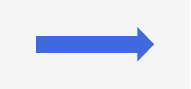
\begin{tikzpicture}
	\color{light-azul}
	\draw[-{Triangle[width=12pt,length=6pt]}, line width=6pt](0,0) -- (1.5, 0);
\end{tikzpicture}{\color{light-azul}{\Large #3}}
	}{%
	\end{spacing}
}

\newenvironment{Tasks}[1]{%
	\upshape\begin{spacing}{1.5}
				\centering
		\fcolorbox{black}{white}{
			\parbox{.96\textwidth}{ 
				{
					{\fontfamily{lmr}\selectfont #1}
		}}}
	}{%
	\end{spacing}
}


\providecommand{\H}{\texttt{HackRF~One}}
 
\usepackage{svg} 
\begin{document}
\maketitle
\thispagestyle{fancy}

\clearpage\newpage 

\section*{Concepts: CR -- SDR -- SS}
\begin{DefQuot}{2.1}
{\begin{itemize}
		\item 
\textit{Cognitive Radio}: intelligent processing and flow controlling of wireless communication for effective use of radio resources, and to enable the coexistence between primary and secondary users (cognitive users).
\end{itemize}
}
\end{DefQuot}
\begin{enumerate}
\item Primary User (PU) is a customer of the spectrum band, having a licensed access at any time in a geographical area. Multiple PUs can use the same spectrum simultaneously -- MPU user cognitive radio network.
\item Secondary User (SU or CR) is licensed to access bands of the spectrum when the corresponding PU or multiple PUs are not accessing them. 
\end{enumerate}

The following three features set cognitive radio apart from conventional radio:
\begin{itemize}
	\item
\textsl{Cognition}: CR is aware of its physical and administrative surroundings.
\item
\textsl{Reconfiguration}: This cognitive understanding allows CR to select whether to dynamically and independently change its parameters.
\item
\textsl{Learning}: CR can benefit from the experience and test out new setups in fresh circumstances.
\end{itemize}
\bigskip
\begin{DefQuot}{2.1}
{
\textit{Spectrum Sensing} is the process of gaining an understanding of the state of channel occupancy and identifying the existence of spectrum holes in a geographical area before a transmission is initiated. 

The spectrum sensing problem is defined as a hypotheses test based on the presence of the primary user signal:

 \begin{itemize}
 	\item $H_0$: No primary user signal is present (absence)
 	
 	\item $H_1$: primary user signal is present (presence)
 \end{itemize}
}
\end{DefQuot}
\clearpage\newpage 

\section{\Large{SDR-based~Testbed~Environment}}

\begin{DefQuot}{1.2}
	{\textit{Software-Defined Radio} is a radio communication system in which any physical item or function can be performed or automated by software. Thus, SDR replaces traditional hardware components through software algorithms, enhancing flexibility and adaptability in radio systems, and enabling the development of CR prototypes and solutions. The testbed enables evaluation of communication protocols to be implemented in real-world scenarios \href{https://ieeexplore.ieee.org/abstract/document/9989359}{$\textcolor{light-red}{\bullet}$}. 
		
}\end{DefQuot}
 
\begin{figure}[!ht] 
	\centering
	\resizebox{.81\columnwidth}{!}{\setlength{\unitlength}{5400sp}%
\begin{picture}(7200,3000)(720,-2400)
% METADATA <id>190</id> 
\thinlines
{\color{light-olive}\put(6813,-1516){\framebox(857,945){}}
}%
% METADATA <id>203</id> 
{\color{light-olive}\put(7670,-808){\line( 1, 0){125}}
\put(7795,-814){\line( 0, 1){709}}
}%
% METADATA <id>204</id> 
{\color{light-olive}\put(7670,-1281){\line( 1, 0){360}}
\put(8030,-1284){\line( 0, 1){1653}}
}%
% METADATA <id>211</id> 
{\color{light-olive}\put(7683,127){\line( 1, 0){237}}
\multiput(7920,127)(-2.91220,-5.82439){42}{\makebox(1.2723,8.9059){\tiny.}}
\multiput(7795,-109)(-2.84878,5.69756){42}{\makebox(1.2723,8.9059){\tiny.}}
}%
% METADATA <id>202</id> 
{\color{light-olive}\put(6813,-1281){\vector(-1, 0){259}}
}%
 
{\color{light-olive}\put(6554,-808){\vector( 1, 0){236}}
}%
% METADATA <id>209</id> 
{\color[rgb]{0,0,0}\put(4716,-1512){\vector( 0, 1){214}}
}%
% METADATA <id>208</id> 
{\color[rgb]{0,0,0}\put(4716,-577){\vector( 0,-1){214}}
}%
% METADATA <id>200</id> 
% METADATA <link srcPointIdx=1 targetObjId=186 targetLeftPointIdx=3/> 
{\color[rgb]{0,0,0}\put(5539,-1281){\vector(-1, 0){1726}}
}%
% METADATA <id>207</id> 
{\color[rgb]{0,0,0}\put(2121,-1501){\vector( 0, 1){214}}
}%
% METADATA <id>205</id> 
{\color[rgb]{0,0,0}\put(2121,-582){\vector( 0,-1){214}}
}%
% METADATA <id>198</id> 
% METADATA <link srcPointIdx=1 targetObjId=186 targetLeftPointIdx=3/> 
{\color[rgb]{0,0,0}\put(3813,-808){\vector( 1, 0){1726}}
}%
% METADATA <id>192</id> 

\put(3300,210){\makebox(0,0)[lb]{\smash{\fontsize{16}{19.2}\usefont{T1}{ptm}{m}{n}{SDR Functional Diagram}%
}}}

\put(6937,-1281){\makebox(0,0)[lb]{\smash{\fontsize{16}{19.2}\usefont{T1}{ptm}{m}{n}{\color{light-olive}Section}%
}}}
% METADATA <id>195</id> 
\put(7118,-999){\makebox(0,0)[lb]{\smash{\fontsize{16}{19.2}\usefont{T1}{ptm}{m}{n}{\color{light-olive}RF}%
}}}

% METADATA <id>197</id> 
% METADATA <link srcPointIdx=1 targetObjId=23 targetLeftPointIdx=3/> 
\thinlines
{\color[rgb]{0,0,0}\put(2877,-1281){\vector(-1, 0){1703}}
}%

{\color[rgb]{0,0,0}\put(1174,-806){\vector( 1, 0){1703}}
}%
% METADATA <id>186</id> 
{\color{light-olive}\put(5539,-1518){\framebox(1015,947){}}
}%

% METADATA <id>23</id> 
{\color[rgb]{0,0,0}\put(2877,-1516){\framebox(936,945){}}
}%
% METADATA <id>4</id> 
{\color[rgb]{0,0,0}\put( 91,-1518){\framebox(1083,947){}}
}%
% METADATA <id>8</id> 
%{\color[rgb]{0,0,0}\put(1309,-593){\framebox(1466,631){}}
%}%
% METADATA <id>188</id> 
\put(5737,-1324){\makebox(0,0)[lb]{\smash{\fontsize{16}{19.2}\usefont{T1}{ptm}{m}{n}{\color{light-olive}Section}%
}}}
% METADATA <id>189</id> 
\put(5984,-1099){\makebox(0,0)[lb]{\smash{\fontsize{16}{19.2}\usefont{T1}{ptm}{m}{n}{\color{light-olive}IF}%
}}}
% METADATA <id>194</id> 
\put(5696,-852){\makebox(0,0)[lb]{\smash{\fontsize{16}{19.2}\usefont{T1}{ptm}{m}{n}{\color{light-olive}Analog}%
}}}
% METADATA <id>181</id> 
\put(4050,-1680){\makebox(0,0)[lb]{\smash{\fontsize{11}{19.2}\usefont{T1}{ptm}{m}{n}{\color[rgb]{0,0,0}\textsl{Analog/Digital\ Converter}}%
}}}
% METADATA <id>180</id> 
\put(4061,-510){\makebox(0,0)[lb]{\smash{\fontsize{11}{19.2}\usefont{T1}{ptm}{m}{n}{\color[rgb]{0,0,0}\textsl{Digital/Analog\ Converter}}%
}}}

% METADATA <id>197</id> 
\thinlines

{\color[rgb]{0,0,0}\put(1174,-806){\vector( 1, 0){1703}}
}%
% METADATA <id>213</id> 
{\color[rgb]{0,0,0}\put(7918,605){\line( 1, 0){237}}
\multiput(8155,605)(-2.91220,-5.82439){42}{\makebox(1.2723,8.9059){\tiny.}}
\multiput(8030,369)(-2.84878,5.69756){42}{\makebox(1.2723,8.9059){\tiny.}}
}%
% METADATA <id>26</id> 
\put(3035,-1360){\makebox(0,0)[lb]{\smash{\fontsize{16}{19.2}\usefont{T1}{ptm}{m}{n}{\color[rgb]{0,0,0}Section}%
}}}
% METADATA <id>27</id> 
\put(3282,-1135){\makebox(0,0)[lb]{\smash{\fontsize{16}{19.2}\usefont{T1}{ptm}{m}{n}{\color[rgb]{0,0,0}IF}%
}}}
% METADATA <id>24</id> 
\put(3087,-880){\makebox(0,0)[lb]{\smash{\fontsize{14}{19.2}\usefont{T1}{ptm}{m}{n}{\color[rgb]{0,0,0}{Digital}}%
}}}
% METADATA <id>17</id> 
\put(1354,-2014){\makebox(0,0)[lb]{\smash{\fontsize{16}{19.2}\usefont{T1}{ptm}{m}{n}{\color[rgb]{0,0,0}\textsl{down-converter}}%
}}}
% METADATA <id>15</id> 
\put(1766,-1759){\makebox(0,0)[lb]{\smash{\fontsize{14}{19.2}\usefont{T1}{ptm}{m}{n}{\color[rgb]{0,0,0}\textsl{Digital}}%
}}}
% METADATA <id>10</id> 
\put(1475,-491){\makebox(0,0)[lb]{\smash{\fontsize{14}{19.2}\usefont{T1}{ptm}{m}{n}{\color[rgb]{0,0,0}\textsl{up-converter}}%
}}}
% METADATA <id>9</id> 
\put(1760,-221){\makebox(0,0)[lb]{\smash{\fontsize{16}{19.2}\usefont{T1}{ptm}{m}{n}{\color[rgb]{0,0,0}\textsl{Digital}}%
}}}
% METADATA <id>7</id> 
\put(322,-1383){\makebox(0,0)[lb]{\smash{\fontsize{16}{19.2}\usefont{T1}{ptm}{m}{n}{\color[rgb]{0,0,0}Section}%
}}}
% METADATA <id>6</id> 
\put(215,-1146){\makebox(0,0)[lb]{\smash{\fontsize{16}{19.2}\usefont{T1}{ptm}{m}{n}{\color[rgb]{0,0,0}Baseband}%
}}}
% METADATA <id>5</id> 
\put(362,-887){\makebox(0,0)[lb]{\smash{\fontsize{16}{19.2}\usefont{T1}{ptm}{m}{n}{\color[rgb]{0,0,0}Digital}%
}}}

\thinlines
%  METADATA <id>1</id> 
{\color[rgb]{0,0,0}\put(0,-2490){\vector(-1, 0){  0}}
	\put(0,-2490){\vector( 1, 0){5400}}
}%
\put(1020,-2400){\makebox(0,0)[lb]{\smash{\fontsize{16}{19.2}\usefont{T1}{ptm}{m}{n}{\color[rgb]{0,0,0}\textsl{Discrete/Digital Signal Processing}}%
}}}
{\color{light-olive}\put(5580,-2490){\vector(-1, 0){  0}}
	\put(5580,-2490){\vector( 1, 0){2100}}
}%
\put(5910,-2400){\makebox(0,0)[lb]{\smash{\fontsize{16}{19.2}\usefont{T1}{ptm}{m}{n}{\color{light-olive}\textsl{Analog Processing}}%
}}}

\put(6000,-90){\makebox(0,0)[lb]{\smash{\fontsize{11}{19.2}\usefont{T1}{ptm}{m}{n}{\color{light-olive}\textsl{Application Specific}}%
}}}
\put(6000,-300){\makebox(0,0)[lb]{\smash{\fontsize{11}{19.2}\usefont{T1}{ptm}{m}{n}{\color{light-olive}\textsl{Integrated Circuits}}%
}}}
\end{picture}%
 }
%	\caption{SDR functional diagram.}
\end{figure}

\begin{figure}[!ht] 
	\vspace*{1.2cm}
	\centering
	\resizebox{.84\columnwidth}{!}{%
%  Created by WinFIG version 2021.1 
%  METADATA <version>1.0</version> 
%
\setlength{\unitlength}{3947sp}%
%
\begingroup\makeatletter\ifx\SetFigFont\undefined%
\gdef\SetFigFont#1#2#3#4#5{%
  \reset@font\fontsize{#1}{#2pt}%
  \fontfamily{#3}\fontseries{#4}\fontshape{#5}%
  \selectfont}%
\fi\endgroup%
\begin{picture}(6339,2250)(114,-1650)
%  METADATA <id>1</id> 
\thicklines
{\color{light-olive}\put(474,-1059){\framebox(1185,1425){}}
}%
%  METADATA <id>2</id> 
\thinlines
{\color{light-olive}\put(699,-811){\framebox(712,712){}}
}%
%  METADATA <id>10</id> 
{\color[rgb]{0,0,0}\put(2619,-833){\framebox(712,712){}}
}%
%  METADATA <id>16</id> 
{\color[rgb]{0,0,0}\put(3324,-331){\vector(-1, 0){  0}}
\put(3324,-331){\vector( 1, 0){457}}
}%
%  METADATA <id>17</id> 
{\color[rgb]{0,0,0}\put(3781,-826){\framebox(938,967){}}
}%
%  METADATA <id>18</id> 
{\color[rgb]{0,0,0}\put(4742,-346){\vector(-1, 0){  0}}
\put(4742,-346){\vector( 1, 0){457}}
}%
%  METADATA <id>19</id> 
{\color[rgb]{0,0,0}\put(5214,-826){\framebox(938,967){}}
}%
%  METADATA <id>23</id> 
\thicklines
{\color[rgb]{0,0,0}\put(2626,-1074){\framebox(3795,1425){}}
}%
%  METADATA <id>8</id> 
\thinlines
{\color[rgb]{0,0,0}\put(1951,-137){\line( 0,-1){473}}
\put(1959,-610){\line(-1, 1){248}}
\put(1711,-362){\line( 1, 1){240}}
}%
%  METADATA <id>9</id> 
{\color[rgb]{0,0,0}\put(2349,-137){\line( 0,-1){473}}
\put(2341,-610){\line( 1, 1){248}}
\put(2589,-362){\line(-1, 1){240}}
}%
%  METADATA <id>27</id> 
{\color{light-olive}\multiput(136,603)(3.10345,-7.75862){30}{\makebox(1.6667,11.6667){\tiny.}}
\multiput(226,378)(4.42941,7.38236){31}{\makebox(1.6667,11.6667){\tiny.}}
\put(353,603){\line(-1, 0){225}}
}%
%  METADATA <id>25</id> 
{\color{light-olive}\put(226,366){\line( 0,-1){720}}
\put(226,-354){\line( 1, 0){225}}
}%
%  METADATA <id>28</id> 
\put(540,141){\makebox(0,0)[lb]{\smash{{\SetFigFont{9}{10.8}{\rmdefault}{\mddefault}{\updefault}{\color{light-olive}SDR Platform}%
}}}}
%  METADATA <id>21</id> 
\thicklines
{\color[rgb]{0,0,0}\put(1959,-347){\line( 1, 0){382}}
}%

%  METADATA <id>29</id> 
{\color{light-olive}\put(241,-1531){\vector(-1, 0){  0}}
	\put(241,-1531){\vector( 1, 0){2730}}
}%

 %  METADATA <id>30</id> 
 {\color[rgb]{0,0,1}\put(3076,-1531){\vector(-1, 0){  0}}
 	\put(3076,-1531){\vector( 1, 0){3345}}
 }%
 %  METADATA <id>25</id> 
 {\color[rgb]{0,0,0}\put(226,366){\line( 0,-1){720}}
 	\put(226,-354){\line( 1, 0){225}}
 }%
 %  METADATA <id>27</id> 
 {\color[rgb]{0,0,0}\multiput(136,603)(3.10345,-7.75862){30}{\makebox(1.6667,11.6667){\tiny.}}
 	\multiput(226,378)(4.42941,7.38236){31}{\makebox(1.6667,11.6667){\tiny.}}
 	\put(353,603){\line(-1, 0){225}}
 }%
 %  METADATA <id>29</id> 
 {\color[rgb]{0.82, 0.1, 0.26}\put(241,-1531){\vector(-1, 0){  0}}
 	\put(241,-1531){\vector( 1, 0){2730}}
 }% 
\put(1500,-1710){\makebox(0,0)[lb]{\smash{{\SetFigFont{9}{10.8}{\rmdefault}{\mddefault}{\updefault}{{\textcolor{light-red}{Hardware}}%
}}}}}

\put(4200,-1710){\makebox(0,0)[lb]{\smash{{\SetFigFont{9}{10.8}{\rmdefault}{\mddefault}{\updefault}{{\textcolor{light-azul}{Software}}%
}}}}}

\put(2400,600){\makebox(0,0)[lb]{\smash{{\SetFigFont{9}{10.8}{\rmdefault}{\mddefault}{\updefault}{{\color[rgb]{0,0,0} SDR Architecture}%
}}}}}
%  METADATA <id>29</id> 
\put(804,-300){\makebox(0,0)[lb]{\smash{{\SetFigFont{9}{10.8}{\rmdefault}{\mddefault}{\updefault}{\color{light-olive}RF}%
}}}}
\put(720,-540){\makebox(0,0)[lb]{\smash{{\SetFigFont{9}{10.8}{\rmdefault}{\mddefault}{\updefault}{\color{light-olive}Daughter}%
}}}}
\put(804,-780){\makebox(0,0)[lb]{\smash{{\SetFigFont{9}{10.8}{\rmdefault}{\mddefault}{\updefault}{\color{light-olive}Board}%
}}}}
%  METADATA <id>30</id> 
\put(1830,-72){\makebox(0,0)[lb]{\smash{{\SetFigFont{9}{10.8}{\rmdefault}{\mddefault}{\updefault}{\color[rgb]{0,0,0}Eternet}%
}}}}
%  METADATA <id>32</id> 
\put(2700,-300){\makebox(0,0)[lb]{\smash{{\SetFigFont{9}{10.8}{\rmdefault}{\mddefault}{\updefault}{\color[rgb]{0,0,0}SDR}%
}}}}
\put(2700,-540){\makebox(0,0)[lb]{\smash{{\SetFigFont{7}{10.8}{\rmdefault}{\mddefault}{\updefault}{\color[rgb]{0,0,0}Middleware}%
}}}}
%  METADATA <id>33</id> 
\put(3840,-300){\makebox(0,0)[lb]{\smash{{\SetFigFont{9}{10.8}{\rmdefault}{\mddefault}{\updefault}{\color[rgb]{0,0,0}GNU radio}%
}}}}
\put(3840,-540){\makebox(0,0)[lb]{\smash{{\SetFigFont{9}{10.8}{\rmdefault}{\mddefault}{\updefault}{\color[rgb]{0,0,0}Application}%
}}}}
%  METADATA <id>35</id> 
\put(5289,-60){\makebox(0,0)[lb]{\smash{{\SetFigFont{9}{10.8}{\rmdefault}{\mddefault}{\updefault}{\color[rgb]{0,0,0}Python}%
}}}}
\put(5289,-300){\makebox(0,0)[lb]{\smash{{\SetFigFont{9}{10.8}{\rmdefault}{\mddefault}{\updefault}{\color[rgb]{0,0,0}Processing}%
}}}}
\put(5289,-540){\makebox(0,0)[lb]{\smash{{\SetFigFont{9}{10.8}{\rmdefault}{\mddefault}{\updefault}{\color[rgb]{0,0,0}and GUI}%
}}}}
\put(4500,-1006){\makebox(0,0)[lb]{\smash{{\SetFigFont{9}{10.8}{\rmdefault}{\mddefault}{\updefault}{\color[rgb]{0,0,0}Host PC}%
}}}}
\end{picture}%
}
\end{figure}

	\clearpage\newpage
\paragraph*{SDR-based platform}
\begin{description}
	\item[Hardware]\, 
	
	The hardware of a SDR transceiver usually contains components (processing devices) such as a general purpose processor (GPP), digital signal processing (DSP), and Field Programmable Gate Arrays (FPGA). A SDR device employs a reconfigurable hardware that may be programmed over-the-air by software to function under different wireless standards. 
	
\begin{figure}[!ht] 
	\centering
	\resizebox{.57\columnwidth}{!}{
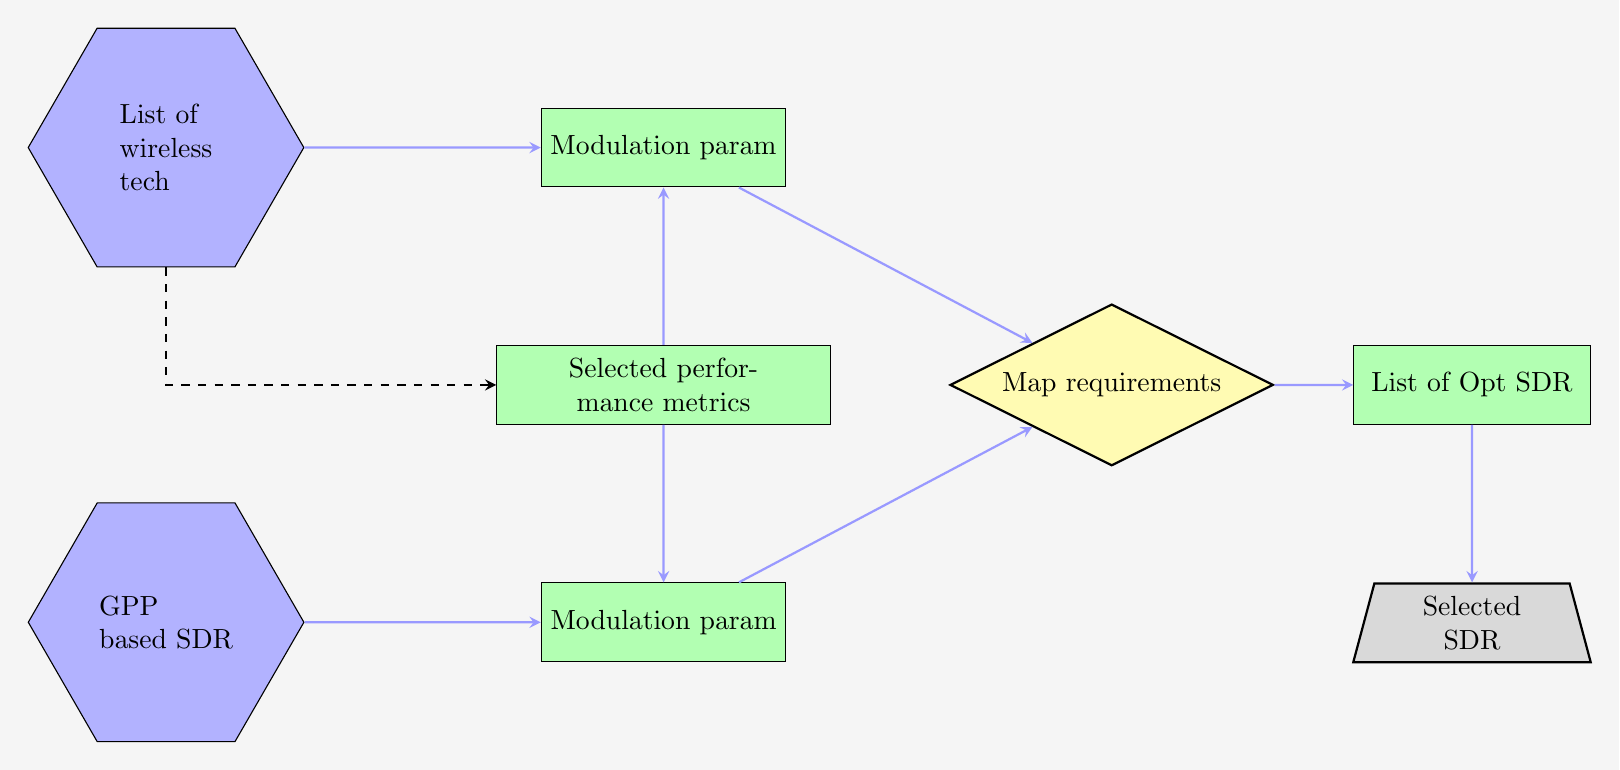
\begin{tikzpicture}[scale=0.8, node distance=2cm and 3cm]  % Escala la gráfica para que encaje en la página

    % Nodes
    \node (wireless_list) [hexagon] {\begin{varwidth}{3cm}
                List of\\
                wireless\\
                tech
            \end{varwidth}
        };
    \node (mod_param1) [block, right=of wireless_list] {Modulation param};
    \node (performance_metrics) [block, below=2cm of mod_param1, text width=4cm] {Selected performance metrics};
    \node (mod_param2) [block, below=2cm of performance_metrics] {Modulation param};
    \node (gpp_sdr) [hexagon, left=3cm of mod_param2]{\begin{varwidth}{3cm}
                GPP\\
                based SDR
            \end{varwidth}
        };
    \node (map_req) [mydiamond, right=of performance_metrics, xshift=-1.5cm] {Map requirements};
    \node (list_opt_sdr) [block, right=of map_req, xshift=-2cm] {List of Opt SDR};
    \node (selected_sdr) [parallelogram, below=2cm of list_opt_sdr, text width=2cm] {Selected SDR};

    % Arrows
    \draw [arrow] (wireless_list) -- (mod_param1);
    \draw [arrow] (mod_param1) -- (map_req);
    \draw [arrow] (performance_metrics) -- (mod_param2);
    \draw [arrow] (gpp_sdr) -- (mod_param2);
    \draw [arrow] (mod_param2) -- (map_req);
    \draw [arrow] (map_req) -- (list_opt_sdr);
    \draw [arrow] (list_opt_sdr) -- (selected_sdr);
    
    % New arrow from "Selected performance metrics" to "Modulation param"
    \draw [arrow] (performance_metrics) -- (mod_param1);
    
    % Dashed arrow
    \draw [dashed_arrow] (wireless_list) |- (performance_metrics);

\end{tikzpicture}

}
	\caption{Selection of SDR Platforms for Wireless Technologies.
		[\href{https://ieeexplore.ieee.org/abstract/document/9721283}{$\gc{\bullet}$}]
	}
\end{figure}

\item[Peripherals] \,

Auxiliary devices for Transmission/Reception of radio signals through reconfigurable hardware components (real-time processing devices, middleware, or Open-source electronic prototyping platforms)

-- \textsl{Antenna Reception System}, determining the signal's propagation characteristics and coverage area. 

--  \textsl{RF Components} such as to filter out unwanted frequencies, and amplify signals to a desired power level. 

\item[Software] \,
	
	%Proprietary software: MATLAB and Simulink / LabVIEW / Xilinx Vivado HLS\newline
	
-- \textsl{ Open source  software}: GNU Radio provides signal-processing blocks that are interconnected to form a flow graph representing the implemented transceiver in software\newline
	
--  \textsl{Third-Party Software} Compatible With HackRF
	 Baseband Data Processing to extract meaningful information through relevant processing based on the application's requirements.	
	
--  \textsl{Control and Monitoring Interfaces} through GUI software, allowing to adjust and optimize TX/RX parameters in varying conditions.
	Post-processing outputs to make available the processed data for use by the application or sending to another system (display, storage unit) for further analysis or
	action.
\end{description}
 
\clearpage\newpage

\subsection{ANE Spectrum Sensing System} 

Spectrum Sensing Bands:
\begin{itemize}
	\item[\gc{Band1}] FM  \rojo{falta} Sub-bands\href{http://spcomnav.uab.es/docs/conferences/Bartolucci_NAVITEC_2016.pdf}{$\gc{\bullet}$} \rojo{falta}
	\item[\gc{Band2}] UHF/VHF TDT \rojo{falta} Sub-bands\href{http://spcomnav.uab.es/docs/conferences/Bartolucci_NAVITEC_2016.pdf}{$\gc{\bullet}$} \rojo{falta}
	\item[\gc{Band3}] L \rojo{falta} Sub-bands\href{http://spcomnav.uab.es/docs/conferences/Bartolucci_NAVITEC_2016.pdf}{$\gc{\bullet}$} \rojo{falta}
	\item[\gc{Band4}] 5G \rojo{falta} Sub-bands\href{http://spcomnav.uab.es/docs/conferences/Bartolucci_NAVITEC_2016.pdf}{$\gc{\bullet}$} \rojo{falta}
\end{itemize}

\medspace
\begin{figure}[!ht] 
	\centering
	\resizebox{.72\columnwidth}{!}{\includegraphics{Figures/MonitoreoMultiBanda.png}}
	\caption{Multiband Spectrum Sensing}
\end{figure}

Spectrum Sensing Networks:

\begin{itemize}
	\item[\gc{SSN1}] FM  \&  \rojo{falta}. 
	\item[\gc{SSN1}] \rojo{falta}
	\item[\gc{SSN3}] \rojo{falta}
\end{itemize}
\clearpage\newpage
\subsection{SDR-based Spectrum Sensing Platform} 
\begin{figure}[!ht] 
	\centering
	\resizebox{\columnwidth}{!}{%
%  Created by WinFIG version 2021.1 
%  METADATA <version>1.0</version> 
%
{\pgfkeys{/pgf/fpu/.try=false}%
\ifx\XFigwidth\undefined\dimen1=0pt\else\dimen1\XFigwidth\fi
\divide\dimen1 by 9249
\ifx\XFigheight\undefined\dimen3=0pt\else\dimen3\XFigheight\fi
\divide\dimen3 by 1194
\ifdim\dimen1=0pt\ifdim\dimen3=0pt\dimen1=3946sp\dimen3\dimen1
  \else\dimen1\dimen3\fi\else\ifdim\dimen3=0pt\dimen3\dimen1\fi\fi
\tikzpicture[x=+\dimen1, y=+\dimen3]
{\ifx\XFigu\undefined\catcode`\@11
\def\temp{\alloc@1\dimen\dimendef\insc@unt}\temp\XFigu\catcode`\@12\fi}
\XFigu3946sp
% Uncomment to scale line thicknesses with the same
% factor as width of the drawing.
%\pgfextractx\XFigu{\pgfqpointxy{1}{1}}
\ifdim\XFigu<0pt\XFigu-\XFigu\fi
\pgfdeclarearrow{
  name = xfiga0,
  parameters = {
    \the\pgfarrowlinewidth \the\pgfarrowlength \the\pgfarrowwidth},
  defaults = {
	  line width=+7.5\XFigu, length=+120\XFigu, width=+60\XFigu},
  setup code = {
    % miter protrusion = thk * sqrt(wd^2 + (tipmv*len)^2) / (2 * wd)
    \dimen7 2.15\pgfarrowlength\pgfmathveclen{\the\dimen7}{\the\pgfarrowwidth}
    \dimen7 2\pgfarrowwidth\pgfmathdivide{\pgfmathresult}{\the\dimen7}
    \dimen7 \pgfmathresult\pgfarrowlinewidth
    \pgfarrowssettipend{+\dimen7}
    \pgfarrowssetbackend{+-\pgfarrowlength}
    \dimen9 -0.5\pgfarrowlinewidth
    \pgfarrowssetvisualbackend{+\dimen9}
    \pgfarrowssetlineend{+-0.5\pgfarrowlinewidth}
    \pgfarrowshullpoint{+\dimen7}{+0pt}
    \pgfarrowsupperhullpoint{+-\pgfarrowlength}{+0.5\pgfarrowwidth}
    \pgfarrowssavethe\pgfarrowlinewidth
    \pgfarrowssavethe\pgfarrowlength
    \pgfarrowssavethe\pgfarrowwidth
  },
  drawing code = {\pgfsetdash{}{+0pt}
    \ifdim\pgfarrowlinewidth=\pgflinewidth\else\pgfsetlinewidth{+\pgfarrowlinewidth}\fi
    \pgfpathmoveto{\pgfqpoint{-\pgfarrowlength}{0.5\pgfarrowwidth}}
    \pgfpathlineto{\pgfqpoint{0pt}{0pt}}
    \pgfpathlineto{\pgfqpoint{-\pgfarrowlength}{-0.5\pgfarrowwidth}}
    \pgfusepathqstroke
  }
}
\clip(150,-1800) rectangle (9600,-150);
\tikzset{inner sep=+0pt, outer sep=+0pt}
%  METADATA <id>2</id> 
\pgfsetlinewidth{+7.5\XFigu}
\pgfsetdash{}{+0pt}
\pgfsetstrokecolor{red}
\draw (180,-210) rectangle (4850,-1770);
%  METADATA <id>3</id> 
\pgftext[base,left,at=\pgfqpointxy{1800}{-360}] {\fontsize{12}{14.4}\usefont{T1}{ptm}{m}{n}\textcolor{light-red}{Hardware}}
\pgfsetstrokecolor{blue}
\draw (4880,-210) rectangle (9510,-1770);
\pgftext[base,left,at=\pgfqpointxy{6000}{-360}] {\fontsize{12}{14.4}\usefont{T1}{ptm}{m}{n}\textcolor{light-azul}{Software}}
\pgfsetstrokecolor{black}
\draw (225,-450) rectangle (2355,-1620);
%  METADATA <id>3</id> 
\draw (2625,-450) rectangle (4755,-1620);
%  METADATA <id>4</id> 
\draw (4980,-450) rectangle (7110,-1620);
%  METADATA <id>5</id> 
\draw (7320,-450) rectangle (9450,-1620);
%  METADATA <id>10</id> 
\pgfsetarrows{[line width=7.5\XFigu]}
\pgfsetarrowsend{xfiga0}
\pgfsetstrokecolor{blue}
\draw (2355,-1065)--(2610,-1050);
%  METADATA <id>11</id> 
\draw (4740,-1065)--(4995,-1050);
%  METADATA <id>12</id> 
\draw (7095,-1035)--(7350,-1020);
%  METADATA <id>6</id> 
\pgfsetfillcolor{black}
\pgftext[base,left,at=\pgfqpointxy{480}{-1020}] {\fontsize{12}{14.4}\usefont{T1}{ptm}{m}{n}Data acquisition}
\pgftext[base,left,at=\pgfqpointxy{480}{-1350}] {\fontsize{12}{14.4}\usefont{T1}{ptm}{m}{n}\& Peripherals}

%  METADATA <id>7</id> 
\pgftext[base,left,at=\pgfqpointxy{2940}{-1020}] {\fontsize{12}{14.4}\usefont{T1}{ptm}{m}{n}Signal Processing }
\pgftext[base,left,at=\pgfqpointxy{2940}{-1350}] {\fontsize{12}{14.4}\usefont{T1}{ptm}{m}{n}\& Radio Scanning }
%  METADATA <id>8</id> 
\pgftext[base,left,at=\pgfqpointxy{5205}{-1020}] {\fontsize{12}{14.4}\usefont{T1}{ptm}{m}{n}Database System}
\pgftext[base,left,at=\pgfqpointxy{5205}{-1350}] {\fontsize{12}{14.4}\usefont{T1}{ptm}{m}{n}\& Management}
%  METADATA <id>9</id> 
\pgftext[base,left,at=\pgfqpointxy{7590}{-1020}] {\fontsize{12}{14.4}\usefont{T1}{ptm}{m}{n}Visualization}
\pgftext[base,left,at=\pgfqpointxy{7590}{-1350}] {\fontsize{12}{14.4}\usefont{T1}{ptm}{m}{n}Dashboards}
\endtikzpicture}%
}
	\caption{Spectrum Sensing Prototype}
\end{figure}	

 \paragraph{Data Acquisition \& Peripherals} 
	\begin{itemize}
		\item SDR Hardware: \newline
	{\color[rgb]{0,.5,0}{\checkmark}} SDR Dongle: \texttt{HackRF~One}
	
	\begin{table}[!ht]
		\centering
		\small
		\begin{tabular*}{.9\columnwidth}{@{\extracolsep{\fill}} |l|lllll|}
			%\begin{tabular}{|l|l|l|l|l|l|}
			\hline
			~ & \textbf{USRP}	
			B210 & \textbf{LimeSDR} & \gc{\texttt{HackRF~One}} & \textbf{ADALM		
				Pluto} & \textbf{RTL-SDR} \\ \hline
			\textsl{RF Range} & 70MHz-6GHz & 100kHz-3.8GHz & 1MHz-6GHz & 325MHz-3.8/6GHz & 500kHz-1.766GHz \\ 
			\textsl{Bandwidth} & 61.44 MHz & 61.44 MHz & 20 MHz & 20 MHz & 2.4 MHz \\ 
			\textsl{ADC} & 12 bits & 12 bits & \gc{8 bits}\footnote{1. Poor representation format} & 12 bits & 8 bits \\
			\textsl{MIMO} & $2\times2$ & $2\times2$ & \gc{none}\footnote{2. direct diversity reception excluded} & none & none \\
			\textsl{FPGA} & Xilinx		
			Spartan-6 & Altera	
			Cyclone IV & \gc{none}\footnote{3. Poor processing capability} & Xilinx Zynq		
			Z-7010 & none \\ \hline
		\end{tabular*}
		\caption{Available SDR platforms}
		{ 1. Poor representation format\newline
			2. Straightforward diversity reception excluded\newline
			3. Poor processing capability\newline
		}
	\end{table}
	
		\halfcheckmark PC's sound card (ADC/DAC + PC processing ) is free and easier to use for RF experimentation.
		
		\Cross Maia SDR that is a portable solution using Web-based interface  accessed from a smartphone, PC or other device. \href{https://maia-sdr.org/}{$\rojo{\bullet}$}
		\item
		SW for Supporting SDR: 
		\begin{list}{*}{}
			\item Drivers and Libraries to interface with the \texttt{HackRF~One} SDR:  
			
			{\color[rgb]{0,.5,0}{\checkmark}} GNU Radio\footnote{GNU Radio is a free \& open-source software development toolkit that provides signal processing blocks to implement SDR designs}
			%Windows: SDR\# (SDRSharp) is very popular and user-friendly.Linux/macOS: GQRX or CubicSDR are good choices.
			\item Programming Environment: 
			
			\Cross PySDR. For mastering topics in the areas of DSP, SDR, and wireless communications \href{https://pysdr.org/index.html}{$\rojo{\bullet}$}. 	
				
			{\color[rgb]{0,.5,0}{\checkmark}} Python. Collab\href{https://colab.research.google.com/}{$\rojo{\bullet}$} Deepnote \href{https://colab.research.google.com/}{$\rojo{\bullet}$}	
					
			{\color[rgb]{0,.5,0}{\checkmark}}  Qt cross-platform C++  [for fast low-level processing] \href{https://deepnote.com/}{$\rojo{\bullet}$}. 	
			
		\end{list}
\clearpage\newpage
				\textcolor{light-olive}{GNU Radio (Python Script))} of installing libraries for \texttt{HackRF~One}\href{https://deepnote.com/workspace/german-castellanos-dominguez-6c6a-246f99fc-b475-4d54-9a79-81e3601710af/project/ANE-8875a419-1789-4110-9f86-9e57021c79b7/notebook/DA001-ef65d5d92f91453d9b7efdebb3c8beb4}{$\textcolor{light-olive}{\bullet}$}. 
				
		\begin{python}
			pip install pyhackrf
		\end{python}

		\begin{python}
			# Spectrum Sensing Script
			
			import numpy as np              		# numerical operations
			import matplotlib.pyplot as plt 		# visualization
			from   pyhackrf import HackRF
			
			def main():
				# Initialize HackRF
				hackrf = HackRF()					# Initialize the SDR device.
			
				try:
					# Configure HackRF
					hackrf.sample_rate = 20e6	    # Set the sample rate to 2.4 MHz
					hackrf.center_freq = 100e6      # Set the center frequency to 100 MHz
					hackrf.gain = 40                # Gain level can be adjusted as needed
					#hackrf.gain = 'auto'           # Automatically adjust the gain.
			
					# Read samples
					print("Reading samples from HackRF...")
					samples = hackrf.read_samples(1024*1024) 
					# Read 1M samples
			
				finally:
					# Ensure the HackRF is properly closed
					hackrf.close()
			
				if __name__ == "__main__":
					main()	
		\end{python}
		
		\item Antenna Reception Array
		\begin{list}{*}{}	
			
			\item \textsl{Single Antenna Reception}. Direct connection to \texttt{HackRF~One} having a single RF input/output 
			\begin{list}{**}{}
				\item \gc{Band1}:
				{\color[rgb]{0,.5,0}{\checkmark}} Omni-Directional FM Reception Antenna. $$\textrm{Element Length}[m] {=} 75/Fo [MHz]=[0.68{-}0.86] [m] {->} 0.75 m$$	
				\halfcheckmark  High Gain Omni-Directional FM Reception Antenna
				\href{https://www.ebay.com/itm/223067751975?_nkw=Fm+Yagi+Antenna&itmmeta=01J63GC1XRQ1TP457QQEGTPA18&hash=item33efdfc627:g:4TMAAOSwP1JbUJj5&itmprp=enc%3AAQAJAAAA8HoV3kP08IDx%2BKZ9MfhVJKnUwTQyIJVYaOllyVytv6R5efqysqSDYWbS%2BQAoVFWBJxESPaxxYbYxunFuqgy4MtknKUu9nwTedKvMogd6clFZO6Bh1vxpobKyfrkBC4f77xeNmoOo2OT8spZTOGIuyxTi%2FuNEFWjPi9zc2ciyVpAX1EAYk4f4kfr%2FWb%2B8zEEM%2Fv00VuqDxeId5KhtNA8hqjUjTL%2F1vhnnxgQXELVy36%2BNRAbgTbQw2wo0PqNmyvIvI374TYT%2FCEakSfaqFSBm4ph8vuvo4W5hPDkjwtvoSllOmkB5BnJfvnItuLOtNp8D5Q%3D%3D%7Ctkp%3ABFBM-p6w8LBk}{$\gc{\bullet}$}\newline 			
				\Cross Dipole Antenna Kit. \href{https://www.ebay.com/itm/184454035475?_nkw=Fm+Yagi+Antenna&itmmeta=01J63GC1XRV3Y6SWX44DXMQ751&hash=item2af2513813:g:4DcAAOSwLOlfaeIw&itmprp=enc%3AAQAJAAAA0HoV3kP08IDx%2BKZ9MfhVJKmJHCtCOF8UeY%2Bb%2Fy6iTONEDTwT0yam59lHnA3YbV2Ypg5hf%2BP%2BimO43wWQ7uhyafChSNRzMo%2BMHWvfihqTsx0ha4w6dvOW7IMtfw6l4atlUdv5MGeWldUGneRwiuymBamAqggl9q0Dqoxpo527mPIRRq092fl6kMZco0yrQgXq8nb65hvIPfcv0rzoVp%2BhkljDakiVvOcKav%2BZSu3goKWUTqxvJF7FZqdkfZvzyMtkFHJFIubEytPslY%2BTK6hlTIM%3D%7Ctkp%3ABk9SR_yesPCwZA}{$\gc{\bullet}$}
				
				\item \gc{Band2}: 		
				{\color[rgb]{0,.5,0}{\checkmark}}  Omni-Directional FM Reception Antenna.\newline
				\halfcheckmark 
				VHF band Omni-Directional Reception Antenna.\newline			
				\Cross Yagi Antenna, Discone Antenna, Log-Periodic Antenna, vertical ground plane antenna 			
				\item \gc{Band3}: 
				{\color[rgb]{0,.5,0}{\checkmark}}  \rojo{falta}.
				\item \gc{Band4}: 
				{\color[rgb]{0,.5,0}{\checkmark}}  \rojo{falta}.
				\item \gc{Band5}: 
				{\color[rgb]{0,.5,0}{\checkmark}}  \rojo{falta}.
			\end{list}
				
			\item \Cross \textsl{Two separate \texttt{HackRF~One} devices + Synchronization.} Each SDR is connected to a separate antenna, involving external clock sources or custom synchronization circuits (e.g., for MIMO or coherent signal processing), as \texttt{HackRF~One} does not natively support phase synchronization across multiple units. 
			\item \halfcheckmark  \textsl{Dual antenna time-multiplexed SDR system.} Two antennas are used in conjunction with a time multiplexing technique to share resources such as a single SDR receiver or transmitter. Synchronization is also required by Software Integration. Time-division multiplexing is used to alternate between the two antennas, allowing each to transmit or receive signals in different time slots, without the need for two separate SDR channels.
			
			\begin{figure}[!ht] 
				\centering
				\resizebox{.72\columnwidth}{!}{\includegraphics{Figures/AntennaMux.png}}
				\caption{Antenna Multiplex System\href{https://www.ursi.org/proceedings/procGA02/papers/p1879.pdf}{$\gc{\bullet}$}}
			\end{figure}
			
			\textcolor{light-olive}{GNU Radio (Python Script)
			\href{https://deepnote.com/workspace/german-castellanos-dominguez-6c6a-246f99fc-b475-4d54-9a79-81e3601710af/project/ANE-8875a419-1789-4110-9f86-9e57021c79b7/notebook/DA002-8a9fa3f33b8642bea091b21c66a08eea}{${\bullet}$}}. 
			
Considerations:\newline
Time Accuracy: Depending on your application,  more precise control over time multiplexing maybe needed.  timers or hardware interrupts are used to ensure accurate time control.\newline
Antenna Latency Switching: Some SDR devices have delays when switching antennas. The switching time for your hardware must be tested to ensure it meets MUX requirements.
			
\item {\color[rgb]{0,.5,0}{\checkmark}} \textsl{Dual Antenna Switch} \href{https://www.dxengineering.com/parts/dmn-cx310a}{$\gc{\bullet}$}.
		  An external RF switch controlled by an Raspberry Pi GPIO on the \texttt{HackRF~One} is  used to toggle between two antennas connected to the RF switch.  \texttt{HackRF~One} has four GPIO pins (labeled GPIO4, GPIO5, GPIO6, and GPIO7)   used to control external hardware like an RF switch.
		  
		  \textcolor{light-olive}{GNU Radio (Python Script)
		  	\href{https://deepnote.com/workspace/german-castellanos-dominguez-6c6a-246f99fc-b475-4d54-9a79-81e3601710af/project/ANE-8875a419-1789-4110-9f86-9e57021c79b7/notebook/DA003-9da262e37be94cb29a1bf117b44f8bdd}{${\bullet}$}}. 		  
 
Consideration\newline
Depending on each application, the switching time may be a concern. Some RF switches might have delays or require debounce logic, especially for fast switching applications.

Enhanced Reception
\begin{list}{**}{}
	\item  Two omni-antennas for Diversity Reception or Scanning Different Bands \gc{Band1}, \gc{Band4}\rojo{falta}
	\item Two Directional Signal Analysis (one directional antenna (e.g., Yagi) towards a specific signal source, while the other (e.g., omnidirectional) covers a broader area)  \gc{Band2}\rojo{falta}
	\item FM DX to receive distant or rare FM stations, including the use of UAV. \gc{Band1}  	\rojo{falta}
\end{list}  
\end{list}
\item \halfcheckmark Antenna Rotator to monitor stations from different directions, allowing to remotely adjust the antenna's direction. Controlling an antenna rotator typically involves interfacing with external hardware via protocols like Yaesu GS-232, DC motor control (e.g., using an  Raspberry Pi), or some specific serial interface to rotate the antenna to a desired azimuth and/or elevation.

Python Code to Control Antenna Rotator:
\textcolor{light-olive}{GNU Radio (Python Script)
	\href{https://deepnote.com/workspace/german-castellanos-dominguez-6c6a-246f99fc-b475-4d54-9a79-81e3601710af/project/ANE-8875a419-1789-4110-9f86-9e57021c79b7/notebook/DA004-45f08e847b884f5ba53bd5e34283e289}{${\bullet}$}}. 

Considerations:\newline
Precision Control of the rotator to accurately respond to azimuth commands. Some rotators may have slight delays, so you  there is a need for experimenting with time.sleep() to give the rotator enough time to move.\newline
Signal Strength Integration  by processing the HackRF's received samples after each rotation to decide if further adjustments are needed.

\item {\color[rgb]{0,.5,0}{\checkmark}}  Multi Sensor GPS-based Synchronization 
\href{http://spcomnav.uab.es/docs/conferences/Bartolucci_NAVITEC_2016.pdf}{$\gc{\bullet}$} 

\begin{figure}[!ht] 
	\centering
	\resizebox{.9\columnwidth}{!}{ 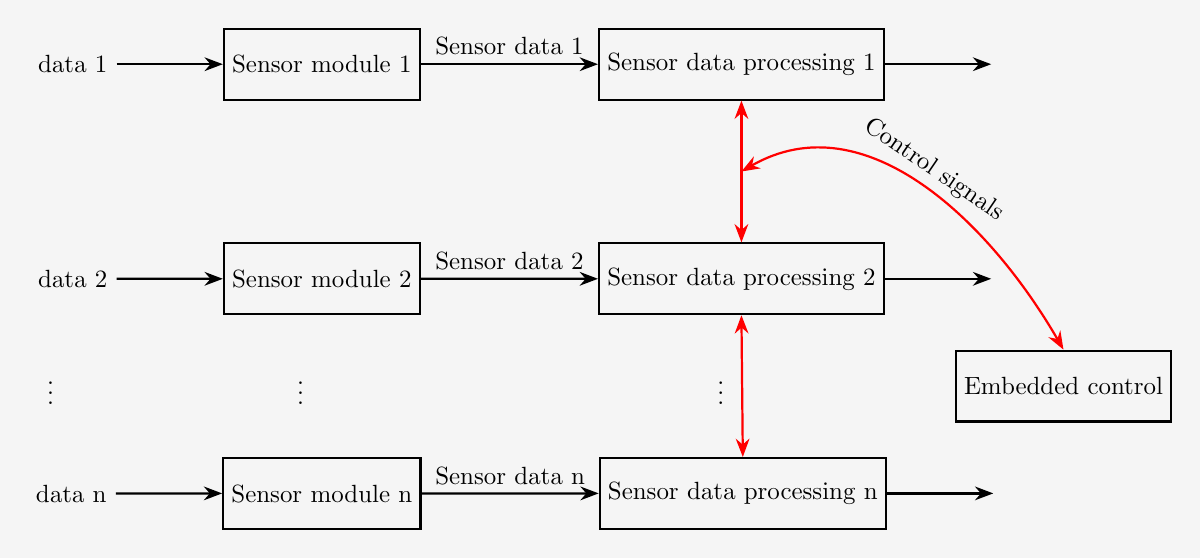
\begin{tikzpicture}[node distance=2cm and 2.5cm, >=Stealth, thick, scale=0.9, transform shape]

    % Nodes
    \node (sensor1) [draw, rectangle, minimum width=2.5cm, minimum height=1cm] {Sensor module 1};
    \node (data1) [left=1.5cm of sensor1] {data 1};
    \node (proc1) [right=2.5cm of sensor1, draw, rectangle, minimum width=2.5cm, minimum height=1cm] {Sensor data processing 1};
    
    \node (sensor2) [below=2cm of sensor1, draw, rectangle, minimum width=2.5cm, minimum height=1cm] {Sensor module 2};
    \node (data2) [left=1.5cm of sensor2] {data 2};
    \node (proc2) [right=2.5cm of sensor2, draw, rectangle, minimum width=2.5cm, minimum height=1cm] {Sensor data processing 2};

    \node (sensorn) [below=2cm of sensor2, draw, rectangle, minimum width=2.5cm, minimum height=1cm] {Sensor module n};
    \node (datan) [left=1.5cm of sensorn] {data n};
    \node (procn) [right=2.5cm of sensorn, draw, rectangle, minimum width=2.5cm, minimum height=1cm] {Sensor data processing n};
    
    % Embedded control node (centered between proc2 and procn)
    \node (control) [right=3cm of $(proc2)!0.5!(procn)$, draw, rectangle, minimum width=2.5cm, minimum height=1cm] {Embedded control};

    % Black arrows for outgoing data
    \draw[->] (data1) -- (sensor1);
    \draw[->] (sensor1) -- node[above] {Sensor data 1} (proc1);
    \draw[->] (proc1.east) -- ++(1.5cm, 0);

    \draw[->] (data2) -- (sensor2);
    \draw[->] (sensor2) -- node[above] {Sensor data 2} (proc2);
    \draw[->] (proc2.east) -- ++(1.5cm, 0); % La flecha negra que sale de Sensor data processing 2
    
    \draw[->] (datan) -- (sensorn);
    \draw[->] (sensorn) -- node[above] {Sensor data n} (procn);
    \draw[->] (procn.east) -- ++(1.5cm, 0);

    % Double-headed red arrow between Sensor data processing 1 and Sensor data processing 2
    \draw[<->, red, thick] (proc1.south) -- (proc2.north);

    % Double-headed red arrow between Sensor data processing 2 and Sensor data processing n
    \draw[<->, red, thick] (proc2.south) -- (procn.north);

    % Double-headed red curved arrow from the midpoint of the double-headed arrow between Sensor data processing 1 and Sensor data processing 2
    \draw[<->, red, thick] ($(proc1.south)!0.5!(proc2.north)$) to[out=30, in=120] node[midway, sloped, above, black] {Control signals} (control.north);

  

    % Puntos suspensivos (Ellipsis) sobre los nodos Sensor module n, Sensor data n, Sensor data processing n,
    % corridos ligeramente a la izquierda (-0.3cm en el eje X)
    \node at ($(sensor2)!0.5!(sensorn)+(-0.3cm,0)$) {\vdots};
    \node at ($(data2)!0.5!(datan)+(-0.3cm,0)$) {\vdots};
    \node at ($(proc2)!0.5!(procn)+(-0.3cm,0)$) {\vdots};
    

\end{tikzpicture}

 }
	\caption{Global Synch Scheme}
\end{figure}
\end{itemize} 
\textcolor{light-olive}{GNU Radio for GPS-based Synchronization (Python Script)
	\href{https://github.com/gnss-sdr/gnss-sdr}{${\bullet}$}}. 
\clearpage\newpage

\paragraph{Signal Processing \& Radio Scanning} 
\medspace
\begin{figure}[!ht] 
	\centering		
	%{\resizebox{.57\columnwidth}{!}{\includegraphics{Figures/FreqScanning}}} 
	\resizebox{\columnwidth}{!}{%
%  Created by WinFIG version 2021.1 
%  METADATA <version>1.0</version> 
%
\setlength{\unitlength}{3947sp}%
%
\begingroup\makeatletter\ifx\SetFigFont\undefined%
\gdef\SetFigFont#1#2#3#4#5{%
  \reset@font\fontsize{#1}{#2pt}%
  \fontfamily{#3}\fontseries{#4}\fontshape{#5}%
  \selectfont}%
\fi\endgroup%
\begin{picture}(9000,2250)(-21,-1650)
%  METADATA <id>7</id> 
\thinlines
{\color[rgb]{0,0,0}\put(2131,-1291){\framebox(1170,698){}}
}%
%  METADATA <id>8</id> 
{\color[rgb]{0,0,0}\put(7780,-1037){\framebox(1170,698){}}
}%
%  METADATA <id>9</id> 
{\color[rgb]{0,0,0}\put(4029,-1291){\framebox(1170,698){}}
}%
%  METADATA <id>11</id> 
{\color[rgb]{0,0,0}\put(  1,261){\vector( 1, 0){233}}
}%
%  METADATA <id>21</id> 
{\color[rgb]{0,0,0}\put(3301,-811){\line( 1, 0){510}}
\put(3811,-819){\line( 0, 1){885}}
\put(3819, 66){\vector( 1, 0){180}}
}%
%  METADATA <id>24</id> 
{\color[rgb]{0,0,0}\put(4606,-586){\vector( 0, 1){510}}
}%
%  METADATA <id>25</id> 
{\color[rgb]{0,0,0}\put(8371,-91){\makebox(1.6667,11.6667){\small.}}
}%
%  METADATA <id>26</id> 
{\color[rgb]{0,0,0}\put(8296,-76){\vector( 0,-1){263}}
}%
%  METADATA <id>27</id> 
\put(465,360){\makebox(0,0)[lb]{\smash{{\SetFigFont{9}{10.8}{\rmdefault}{\mddefault}{\updefault}{\color[rgb]{0,0,0}RF/IF Data}%
}}}}
\put(420,180){\makebox(0,0)[lb]{\smash{{\SetFigFont{9}{10.8}{\rmdefault}{\mddefault}{\updefault}{\color[rgb]{0,0,0}Adquisition}%
}}}}
%  METADATA <id>28</id> 
\put(2310,360){\makebox(0,0)[lb]{\smash{{\SetFigFont{9}{10.8}{\rmdefault}{\mddefault}{\updefault}{\color[rgb]{0,0,0}Sampling}%
}}}}
%  METADATA <id>29</id> 
\put(4110,360){\makebox(0,0)[lb]{\smash{{\SetFigFont{9}{10.8}{\rmdefault}{\mddefault}{\updefault}{\color[rgb]{0,0,0}Demodulation}%
}}}}
%  METADATA <id>30</id> 
\put(6000,360){\makebox(0,0)[lb]{\smash{{\SetFigFont{9}{10.8}{\rmdefault}{\mddefault}{\updefault}{\color[rgb]{0,0,0}Spectral and}%
}}}}
\put(6210,180){\makebox(0,0)[lb]{\smash{{\SetFigFont{9}{10.8}{\rmdefault}{\mddefault}{\updefault}{\color[rgb]{0,0,0}PSD }%
}}}}
\put(6000,0){\makebox(0,0)[lb]{\smash{{\SetFigFont{9}{10.8}{\rmdefault}{\mddefault}{\updefault}{\color[rgb]{0,0,0}Estimation}%
}}}}
%  METADATA <id>31</id> 
\put(7890,360){\makebox(0,0)[lb]{\smash{{\SetFigFont{9}{10.8}{\rmdefault}{\mddefault}{\updefault}{\color[rgb]{0,0,0}Parameter}%
}}}}
\put(7890,180){\makebox(0,0)[lb]{\smash{{\SetFigFont{9}{10.8}{\rmdefault}{\mddefault}{\updefault}{\color[rgb]{0,0,0}Calculation}%
}}}}
\put(7890,-690){\makebox(0,0)[lb]{\smash{{\SetFigFont{9}{10.8}{\rmdefault}{\mddefault}{\updefault}{\color[rgb]{0,0,0}Thresholding}%
}}}}
%  METADATA <id>32</id> 
\put(2364,-820){\makebox(0,0)[lb]{\smash{{\SetFigFont{9}{10.8}{\rmdefault}{\mddefault}{\updefault}{\color[rgb]{0,0,0}Frequency}%
}}}}
\put(2364,-1000){\makebox(0,0)[lb]{\smash{{\SetFigFont{9}{10.8}{\rmdefault}{\mddefault}{\updefault}{\color[rgb]{0,0,0}Scaling}%
}}}}
%  METADATA <id>33</id> 
\put(4246,-820){\makebox(0,0)[lb]{\smash{{\SetFigFont{9}{10.8}{\rmdefault}{\mddefault}{\updefault}{\color[rgb]{0,0,0}Frequency}%
}}}}
\put(4246,-1000){\makebox(0,0)[lb]{\smash{{\SetFigFont{9}{10.8}{\rmdefault}{\mddefault}{\updefault}{\color[rgb]{0,0,0}Slotting}%
}}}}

%  METADATA <id>25</id> 
{\color[rgb]{0,0,0}\put(8371,-91){\makebox(1.6667,11.6667){\small.}}
}%
%  METADATA <id>26</id> 
{\color[rgb]{0,0,0}\put(8296,-76){\vector( 0,-1){263}}
}%
%  METADATA <id>6</id> 
{\color[rgb]{0,0,0}\put(7787,-91){\framebox(1170,698){}}
}%
%  METADATA <id>17</id> 
{\color[rgb]{0,0,0}\put(1659,254){\line( 0,-1){1073}}
	\put(1659,-819){\vector( 1, 0){465}}
}%
%  METADATA <id>15</id> 
{\color[rgb]{0,0,0}\put(7089,247){\vector( 1, 0){705}}
}%
%  METADATA <id>14</id> 
{\color[rgb]{0,0,0}\put(5214,247){\vector( 1, 0){705}}
}%
%  METADATA <id>13</id> 
{\color[rgb]{0,0,0}\put(3301,247){\vector( 1, 0){705}}
}%
%  METADATA <id>12</id> 
{\color[rgb]{0,0,0}\put(1411,247){\vector( 1, 0){705}}
}%


%  METADATA <id>5</id> 
{\color[rgb]{0,0,0}\put(5904,-91){\framebox(1170,698){}}
}%
%  METADATA <id>4</id> 
{\color[rgb]{0,0,0}\put(4029,-91){\framebox(1170,698){}}
}%
%  METADATA <id>3</id> 
{\color[rgb]{0,0,0}\put(2131,-91){\framebox(1170,698){}}
}%
%  METADATA <id>2</id> 
{\color[rgb]{0,0,0}\put(241,-91){\framebox(1170,698){}}
}

%  METADATA <id>36</id> 
{\color[rgb]{0,0,0}\put(1890,-1560){\dashbox{45}(1620,2310){}}
}%
\end{picture}%
}
	\caption{Radio Scanning Pipeline}
\end{figure}

\begin{itemize}
	
\item {Sampling}
\begin{list}{.-}{}
	\item
 Sampling Criterion: The sample rate must be at least twice the highest frequency component of the signal to accurately reconstruct the signal without aliasing. For FM radio, the highest frequency component typically includes the carrier frequency plus the deviation caused by the audio signal.
	\item
Bandwidth of FM Signal: FM signals have a wider bandwidth compared to AM signals. The bandwidth is determined by the carrier frequency and the maximum frequency deviation. For commercial FM radio, the bandwidth can be as wide as 200 kHz.

	\item
	Decimation and Interpolation: In SDR systems, the initial sample rate may be very high (e.g., several MHz) to capture a wide range of frequencies. Decimation is used to reduce the sample rate for more manageable processing while preserving the signal of interest. Interpolation can be used to increase the sample rate if necessary for specific processing stages.
\end{list}

\begin{list}{*}{}
\item \gc{Band1}
Typical Sample Rates for FM Demodulation:

.- RTL-SDR: Commonly used SDR hardware like the RTL-SDR typically uses sample rates in the range of 1.024 MSPS (mega samples per second) to 2.048 MSPS. These rates are sufficient to capture the full bandwidth of a commercial FM broadcast.

.- Higher-End SDRs: More advanced SDR hardware can support higher sample rates, providing greater flexibility and the ability to capture wider bandwidths or multiple channels simultaneously.
\begin{python}
	from gnuradio import gr
	from gnuradio import blocks
	from gnuradio import analog
	from gnuradio import filter
	from gnuradio import audio
	
	# Create a flow graph
	fg = gr.top_block()
	
	# Sample rate set high enough to capture the entire FM signal bandwidth (e.g., 2.048 MHz).
	sample_rate = 2.048e6 # 2.048 MHz
	
	# Signal source (e.g., from an RTL-SDR or file)
	src = blocks.file_source(gr.sizeof_gr_complex, "fm_signal.dat", False)
	
	# Throttle block to control the sample rate
	throttle = blocks.throttle(gr.sizeof_gr_complex, sample_rate, True)
	
	# Frequency translating FIR filter to shift the signal to baseband
	freq_trans = filter.freq_xlating_fir_filter_ccc(1, [1], -250e3, sample_rate)
	
	# Low-pass filter to remove high-frequency components
	lpf = filter.fir_filter_ccf(1, filter.firdes.low_pass(1, sample_rate, 100e3, 10e3))
	
	# FM demodulator
	fm_demod = analog.wfm_rcv(
	quad_rate=sample_rate,
	audio_decimation=10,)
	
	# Audio sink to play the demodulated signal
	audio_sink = audio.sink(int(sample_rate / 10), "", True)
	###### The decimation factor is chosen to a manageable level for processing
	## (e.g., reducing from 2.048 MHz to 204.8 kHz with a decimation factor of 10).
	
	# Connect the blocks
	fg.connect(src, throttle, freq_trans, lpf, fm_demod, audio_sink)
	
	# Run the flow graph
	fg.run()
\end{python}


.- \textsl{Initial Sample Rate}: Should be high enough to cover the entire FM signal bandwidth. 2 MHz is a common choice, but it can be adjusted based on the specific requirements of your SDR hardware and the signal environment.

.- \textsl{Audio Sample Rate}: Typically 44.1 kHz or 48 kHz for high-quality audio output.

\begin{python}
from gnuradio import gr
from gnuradio import blocks
from gnuradio import analog
from gnuradio import filter
from gnuradio import audio

# Create a flow graph
fg = gr.top_block()

# Define the initial sample rate (e.g., 2 MHz for capturing the FM signal)
initial_sample_rate = 2e6 # 2 MHz

# Define the audio sample rate (e.g., 48 kHz for audio output)
audio_sample_rate = 48e3 # 48 kHz

# Source block (e.g., from a file or RTL-SDR)
src = blocks.wavfile_source("fm_signal.wav", True)

# Throttle block to control the initial sample rate
throttle = blocks.throttle(gr.sizeof_gr_complex, initial_sample_rate, True)

# Frequency translating FIR filter to shift the signal to baseband
freq_trans = filter.freq_xlating_fir_filter_ccc(1, [1], -250e3, initial_sample_rate)

# Low-pass filter to remove high-frequency components
lpf = filter.fir_filter_ccf(1, filter.firdes.low_pass(1, initial_sample_rate, 100e3, 10e3))

# FM demodulator
fm_demod = analog.wfm_rcv(
quad_rate=initial_sample_rate,
audio_decimation=int(initial_sample_rate / audio_sample_rate),
)

# Audio sink to play the demodulated signal
audio_sink = audio.sink(int(audio_sample_rate), "", True)

# Connect the blocks
fg.connect(src, throttle, freq_trans, lpf, fm_demod, audio_sink)

# Run the flow graph
fg.run()	
\end{python}


\begin{python}
	from gnuradio import gr, blocks, filter, osmosdr
	
	class if_data_sampling(gr.top_block):
	def __init__(self):
	gr.top_block.__init__(self, "IF Data Sampling")
	
	# Parameters
	center_freq = 100e6 # center radio frequency
	if_freq  = 10e6 # center IFrequency
	samp_rate = 2e6  # sampling rate
	
	# SDR Source
	self.src = osmosdr.source(args="numchan=1")
	self.src.set_sample_rate(samp_rate)
	self.src.set_center_freq(center_freq)
	self.src.set_gain(30)
	
	# Downconvert to IF
	self.downconvert = filter.freq_xlating_fir_filter_ccf(1, (1,), if_freq, samp_rate)
	
	# File Sink to store IF data
	self.sink = blocks.file_sink(gr.sizeof_gr_complex, "if_data.bin")
	
	# Connections
	self.connect(self.src, self.downconvert, self.sink)
	
	if __name__ == '__main__':
	tb = if_data_sampling()
	tb.start()
	tb.wait()
\end{python}

The \texttt{Throttling block} is added for controling the flow of data to match the processing rate. 

\begin{python}
from gnuradio import gr, blocks, analog, filter
import osmosdr

class if_data_acquisition(gr.top_block):
 def __init__(self):
  gr.top_block.__init__(self, "IF Data Acquisition")

  # Parameters  
  center_freq = 100e6 # Center Radiofrequency
  if_freq  = 10e6 # Intermediate frequency
  samp_rate = 2e6

  # Blocks
  self.src = osmosdr.source(args="numchan=1")
  self.src.set_sample_rate(samp_rate)
  self.src.set_center_freq(center_freq)
  self.src.set_gain(30)
  self.chan_filt = filter.freq_xlating_fir_filter_ccf(1, (1,), if_freq - center_freq, samp_rate)
  ############ Throttling block
  self.throttle = blocks.throttle(gr.sizeof_gr_complex*1, samp_rate, True)
  self.sink = blocks.file_sink(gr.sizeof_gr_complex*1, "if_data.bin")

  # Connections
  self.connect(self.src, self.chan_filt, self.throttle, self.sink)

if __name__ == '__main__':
 tb = if_data_acquisition()
 tb.start()
 tb.wait()
\end{python}

\clearpage\newpage
Throttling is used to control the rate at which operations are performed, ensuring that the system doesn't get overwhelmed by too many requests in a short period. 
Specific aspects of throttling in SDR:

.- \textsl{Sample Rate Control}: SDR systems often need to process signals at specific sample rates. A throttling block can ensure that samples are produced or consumed at a constant rate, matching the desired sample rate of the system.

.- \textsl{Buffer Management}: In SDR, data is often processed in chunks or buffers. Throttling helps manage these buffers to ensure that they do not overflow (too much data too quickly) or underflow (too little data too slowly).

.- \textsl{Synchronization}: Ensures that different components of the SDR system, which may operate at different rates, remain in sync. For instance, the rate at which data is received from an antenna must be synchronized with the rate at which it is processed and possibly transmitted.

.- \textsl{Flow Graph Control}: In many SDR platforms like GNU Radio, flow graphs (which represent the data flow through various processing blocks) include throttling blocks to control the overall flow of data through the graph. This ensures that each block processes data at the correct rate.

.- \textsl{CPU Load Management}: Throttling can also be used to manage CPU load. By controlling the rate of data processing, the system can avoid overloading the CPU, ensuring stable operation.
\medskip
\begin{python}
from gnuradio import gr
from gnuradio import blocks

# Create a flow graph
fg = gr.top_block()

# Source block generating random data
src = blocks.vector_source_f([1, 0, 1, 0], True)

# Throttle block to limit data flow to 1 sample per second
throttle = blocks.throttle(gr.sizeof_float, 1, True)

# Sink block to print the output
sink = blocks.vector_sink_f()

# Connect the blocks
fg.connect(src, throttle)
fg.connect(throttle, sink)

# Run the flow graph
fg.run()	
\end{python}
\clearpage\newpage

\item
 \gc{Decimation}
 \begin{python}
	from gnuradio import gr, blocks, filter, osmosdr
	
	class if_decimation(gr.top_block):
	 def __init__(self):
	  gr.top_block.__init__(self, "IF Decimation")
	
	  # Parameters
	  
	  center_freq  = 100e6
	  if_freq   = 10e6
	  samp_rate   = 2e6
	  decimation_factor = 10
	
	  # Blocks
	  self.src = osmosdr.source(args="numchan=1")
	  self.src.set_sample_rate(samp_rate)
	  self.src.set_center_freq(center_freq)
	  self.src.set_gain(30)
	
	  # Downconvert to IF
	  self.downconvert = filter.freq_xlating_fir_filter_ccf(1, (1,), if_freq, samp_rate)
	  
	  # Decimate the signal
	  self.decimate = filter.fir_filter_ccf(decimation_factor, (1,))
	  decimated_samp_rate = samp_rate // decimation_factor
	  
	  # Capture decimated IF data
	  self.sink = blocks.file_sink(gr.sizeof_gr_complex, "decimated_if_data.bin")
	
	  # Connections
	  self.connect(self.src, self.downconvert, self.decimate, self.sink)
	
	if __name__ == '__main__':
	 tb = if_decimation()
	 tb.start()
	 tb.wait()
	 \end{python}


Wavelet Decimation 
 \begin{python}
	from gnuradio import gr, blocks, osmosdr
	import pywt
	import numpy as np
	
	class wavelet_decimation(gr.sync_block):
	 def __init__(self, wavelet, level):
	  gr.sync_block.__init__(self,
	   name="wavelet_decimation",
	   in_sig=[np.complex64],
	   out_sig=[np.complex64])
	  self.wavelet = wavelet
	  self.level = level
	
	 def work(self, input_items, output_items):
	  data = input_items[0]
	  coeffs = pywt.wavedec(data, self.wavelet, level=self.level)
	  # Decimate (keep only the approximation coefficients)
	  output_items[0][:] = pywt.waverec(coeffs[:-1] + [None]*self.level, self.wavelet)
	  return len(output_items[0])
	
	class if_wavelet_decimation(gr.top_block):
	 def __init__(self):
	  gr.top_block.__init__(self, "IF Wavelet Decimation")
	
	  # Parameters
	  samp_rate = 2e6
	  center_freq = 100e6
	  wavelet = 'db4'
	  level = 2
	
	  # Blocks
	  self.src = osmosdr.source(args="numchan=1")
	  self.src.set_sample_rate(samp_rate)
	  self.src.set_center_freq(center_freq)
	  self.src.set_gain(30)
	
	  self.wavelet_dec = wavelet_decimation(wavelet, level)
	  
	  self.sink = blocks.file_sink(gr.sizeof_gr_complex, "wavelet_decimated_if_data.bin")
	
	  # Connections
	  self.connect(self.src, self.wavelet_dec, self.sink)
	
	if __name__ == '__main__':
	 tb = if_wavelet_decimation()
	 tb.start()
	 tb.wait()
	
	 \end{python}
	 
 \gc{Frequency scaling} in SDR involves adjusting the sampling rate to match the frequency of interest for effectively capturing and processing signals, especially when dealing with different frequency bands.

\begin{python}
from gnuradio import gr, blocks, analog, filter
import osmosdr

class frequency_scaling(gr.top_block):
 def __init__(self):
  gr.top_block.__init__(self, "Frequency Scaling")

  # Parameters
  samp_rate = 2e6
  center_freq = 100e6
  scaled_samp_rate = 500e3

  # Blocks
  self.src = osmosdr.source(args="numchan=1")
  self.src.set_sample_rate(samp_rate)
  self.src.set_center_freq(center_freq)
  self.src.set_gain(30)

  # Frequency scaling
  self.resampler = filter.rational_resampler_ccf(
   interpolation=int(scaled_samp_rate),
   decimation=int(samp_rate)
  )

  # Sink
  self.sink = blocks.null_sink(gr.sizeof_gr_complex)

  # Connections
  self.connect(self.src, self.resampler, self.sink)

if __name__ == '__main__':
 tb = frequency_scaling()
 tb.start()
 tb.wait()
 
\end{python}
\item  
\gc{Band2} Python Code\rojo{falta}
\item  
\gc{Band3} Python Code\rojo{falta}
\item  
\gc{Band4} Python Code\rojo{falta}

\end{list}
\item Demodulation

Adjusting Input Settings: \rojo{falta tabla por banda}

%.- Reception Mode of \texttt{HackRF~One}: By default, SDR uses heterodyne architecture in the front-end. \newline
.- Bandwidth: $150$\,\textsl{kHz} to capture the full FM signal.\newline
.- Gain Control: Adjust the gain settings within the SDR software to balance signal strength with noise reduction.\newline
.- BB content of fm. Audio + RDS (Radio Data System). Some SDR software can decode RDS, which is the digital information transmitted by FM radio stations, including station names, song information, etc. 

Basic reception structures  to convert RF signals into baseband signals for further processing:
\begin{list}{*}{}
	\item \textsl{Homodyne receiver} (Zero-IF or Direct Conversion)  involves directly converting the RF signal to baseband (DC) without any intermediate frequency stage. It  simplifies the architecture by converting directly to baseband, which is more suited for SDR devices focused on digital signal processing. It provides high sensitivity and better image rejection due to the use of intermediate frequency stages but is more complex.
	
	\begin{figure}[!ht] 
		\centering
		\resizebox{.51\columnwidth}{!}{
			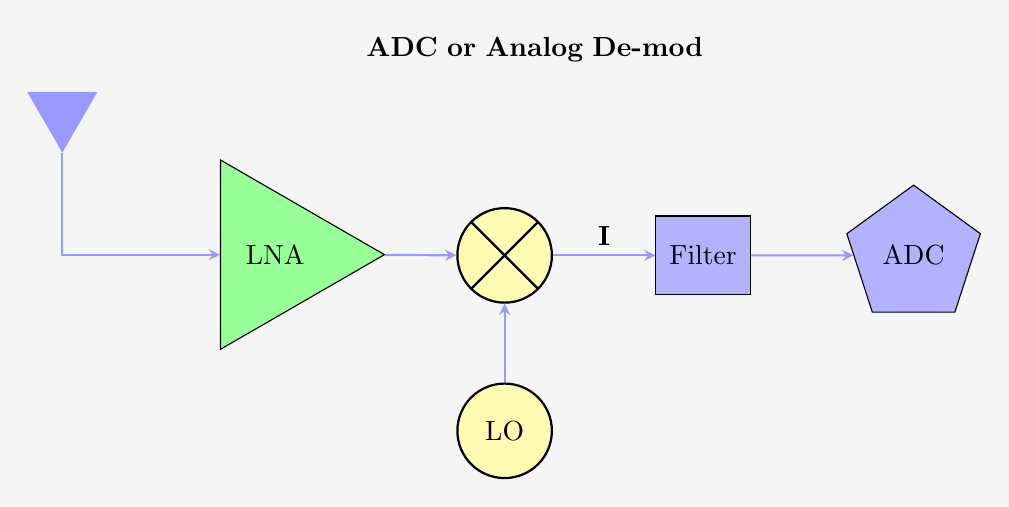
\begin{tikzpicture}[node distance=2cm]
				% Nodes
				\node (antenna) [triangled] {};
				\node (lna) [triangler, fill=green!40, right=2cm of antenna, xshift=1cm, yshift=1cm] {\rotatebox{90}{LNA}};
				\node (multi) [circlex, fill=yellow!30, right=2cm of lna, xshift=0.3cm, yshift=0.8cm]{};
				\node (filter) [box, fill=blue!30, right=2cm of multi, xshift=-0.7cm]{Filter};
				\node (adc) [poligon, fill=blue!30, right=2cm of filter, xshift=-0.7cm]{ADC};
				\node (lo) [circles, fill=yellow!30, below=1cm of multi]{LO};
				\node[textbox] (text1) at (6,0.8) {\textbf{ADC or Analog De-mod}};
				
				% Draws
				\draw [arrow] (antenna) |- (lna);
				\draw [arrow] (lna) -- (multi);
				\draw [arrow] (multi) -- node[anchor=south, black] {\textbf{I}}(filter);
				\draw [arrow] (filter) -- (adc);
				\draw [arrow] (lo) -- (multi);
				
			\end{tikzpicture}
		}
		%	{\resizebox{.21\columnwidth}{!}{\includegraphics{Figures/SDRRX}}} 	
		\caption{Homodyne receiver.}
	\end{figure}
	Drawbacks:\newline
	DC Offset Issues: Direct conversion receivers can suffer from DC offsets, which may interfere with the baseband signal.\newline
	IQ Imbalance: Imperfect in-phase (I) and quadrature (Q) signals can cause IQ imbalance, leading to signal degradation.
	
	\gc{Band1} Python Code\rojo{falta}
	
	\gc{Band2} Python Code\rojo{falta}
	
	\gc{Band3} Python Code\rojo{falta}
	
	\gc{Band4} Python Code\rojo{falta}
	
	\item \textsl{Heterodyne receiver} is the process of converting an incoming high-frequency ($f_{RF}$) signal to an intermediate frequency ($f_{IF}$) before it is down-converted to baseband $f_{BB}$. The  mixer output in a heterodyne receiver is $f_{IF}= \mid f_{RF} -  f_{BB}\mid$
	
	\begin{figure}[!ht] 
		\centering
		\resizebox{.51\columnwidth}{!}{
			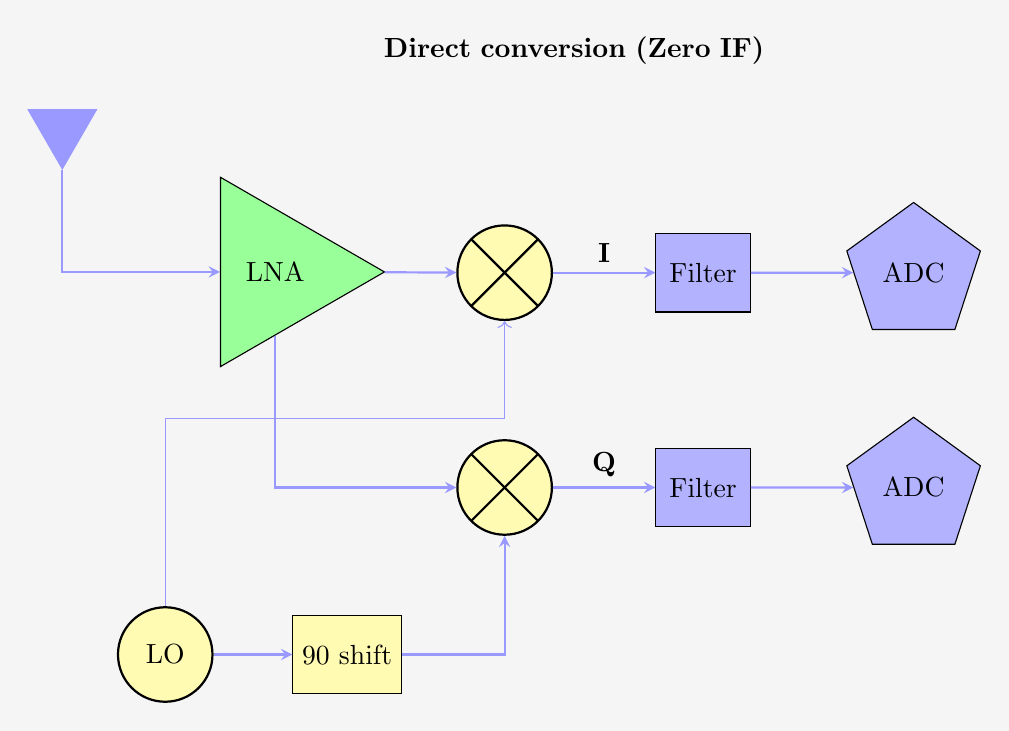
\begin{tikzpicture}[node distance=2cm]
				% Nodes
				\node (antenna) [triangled] {};
				\node (lna) [triangler, fill=green!40, right=2cm of antenna, xshift=1cm, yshift=1cm] {\rotatebox{90}{LNA}};
				\node (multi1) [circlex, fill=yellow!30, right=2cm of lna, xshift=0.3cm, yshift=0.8cm]{};
				\node (filter1) [box, fill=blue!30, right=2cm of multi1, xshift=-0.7cm]{Filter};
				\node (adc1) [poligon, fill=blue!30, right=2cm of filter1, xshift=-0.7cm]{ADC};
				
				\node (multi2) [circlex, fill=yellow!30, below=1.5cm of multi1]{};
				\node (shift) [box, fill=yellow!30, below=1cm of multi2, xshift=-2cm]{90 shift};
				\node (lo) [circles, fill=yellow!30, left=1cm of shift]{LO};
				\node (filter2) [box, fill=blue!30, right=2cm of multi2, xshift=-0.7cm]{Filter};
				\node (adc2) [poligon, fill=blue!30, right=2cm of filter2, xshift=-0.7cm]{ADC};
				\node[textbox] (text1) at (6.5,1) {\textbf{Direct conversion (Zero IF)}};
				
				% Draws
				\draw [arrow] (antenna) |- (lna);
				\draw [arrow] (lna) -- (multi1);
				\draw [arrow] (multi1) -- node[anchor=south, black] {\textbf{I}}(filter1);
				\draw [arrow] (filter1) -- (adc1);
				
				\draw [->, blue!40] (lo) -- ++(0,3) -| (multi1);
				\draw [arrow] (lo) -- (shift);
				\draw [arrow] (shift) -| (multi2);
				\draw [arrow] (multi2) -- node[anchor=south, black] {\textbf{Q}} (filter2);
				\draw [arrow] (filter2) -- (adc2);
				\draw [arrow] (lna) |- (multi2);
				
		\end{tikzpicture}}
		%	{\resizebox{.21\columnwidth}{!}{\includegraphics{Figures/SDRRX}}} 	
		\caption{super heterodyne receiver (a) and homodyne receiver (b).}
	\end{figure}
	
		\gc{Band1} Python Code	\begin{enumerate}
			\item 
			Signal Source captures the signal.
			\item 
			Filtering applies a low-pass filter to isolate the IF signal.
			\item 
			Data Storage the filtered IF data.
		\end{enumerate}
			
	\begin{python}	
		import numpy as np
		import matplotlib.pyplot as plt
		from pyhackrf import HackRF
		from scipy.signal import butter, lfilter
		
		def main():
		# Initialize HackRF
		hackrf = HackRF()
		
		try:
		# Configure HackRF
		hackrf.sample_rate = 20e6  # 20 MHz
		hackrf.center_freq = 100e6 # 100 MHz
		hackrf.gain = 40      # Gain level, can be adjusted as needed
		
		# Read samples
		print("Reading samples from HackRF...")
		samples = hackrf.read_samples(1024*1024) 
		# Read 1M samples
		
		# Demodulate the FM signal
		demodulated_signal = fm_demodulate(samples, hackrf.sample_rate)
		
		finally:
		# Ensure the HackRF is properly closed
		hackrf.close()
		
		def fm_demodulate(samples, sample_rate):
		# Perform quadrature demodulation
		angle = np.angle(samples[1:] * np.conj(samples[:-1]))
		demodulated_signal = np.unwrap(angle)
		
		# Apply low-pass filter
		cutoff_freq = 100e3 # 100 kHz cutoff frequency
		b, a = butter(5, cutoff_freq / (sample_rate / 2), btype='low')
		demodulated_signal = lfilter(b, a, demodulated_signal)
		
		return demodulated_signal
		
		if __name__ == "__main__":
		main()
	\end{python}
	
\end{list}

%\begin{python}
%from gnuradio import gr, blocks, analog, filter
%
%class if_data_acquisition(gr.top_block):
% def __init__(self):
%  gr.top_block.__init__(self, "IF Data Acquisition")
%
%  # Parameters
%  center_freq = 100e6 # center radio frequency
%  samp_rate = 2e6 # sampling rate
%  
%  # Block 1
%  self.src = osmosdr.source(args="numchan=1")
%  self.src.set_sample_rate(samp_rate)
%  self.src.set_center_freq(center_freq)
%  self.src.set_gain(30)
%  # Block 2
%  # Low-pass filter to isolate the IF signal
%  self.lp_filter = filter.fir_filter_ccf(1, filter.firdes.low_pass(
%   1, samp_rate, 200e3, 10e3, filter.firdes.WIN_HAMMING, 6.76))
%  # Block 3
%  # File sink to store the IF data
%  self.file_sink = blocks.file_sink(gr.sizeof_gr_complex*1, "if_data.bin")
%
%  # Connections
%  self.connect(self.src, self.lp_filter, self.file_sink)
%  ######
%if __name__ == '__main__':
% tb = if_data_acquisition()
% tb.start()
% tb.wait()
%\end{python}
 

%\item
 \gc{FM Demodulation}
 
FM Demodulator Block processes the incoming modulated FM signal and converts it into an audio signal.

\begin{python}
from gnuradio import gr
from gnuradio import analog
from gnuradio import blocks
from gnuradio import audio

# Create a flow graph
fg = gr.top_block()

# Source block: A hardware source like RTL-SDR or a simulated source
# For this example, we use a signal source to simulate an FM signal
sample_rate = 250e3 # 250 kHz
signal_freq = 100e3 # 100 kHz
fm_deviation = 75e3 # 75 kHz
audio_rate = 48e3 # 48 kHz (typical audio rate)
fm_signal = analog.sig_source_c(sample_rate, analog.GR_COS_WAVE, signal_freq, 1, 0)

# Throttle block to limit data flow rate
throttle = blocks.throttle(gr.sizeof_gr_complex, sample_rate, True)

# FM Demodulator block
fm_demod = analog.wfm_rcv(
quad_rate=sample_rate,
audio_decimation=int(sample_rate / audio_rate)
)

# Low-pass filter

# Audio sink block
audio_sink = audio.sink(audio_rate, "", True)

# Connect the blocks
fg.connect(fm_signal, throttle)
fg.connect(throttle, fm_demod)
fg.connect(fm_demod, audio_sink)

# Run the flow graph
fg.run()	
\end{python}

Low-Pass Filter for removing high-frequency noise and unwanted components.

\begin{python}
from gnuradio import filter 

# Low-pass filter to remove high-frequency components
lpf = filter.fir_filter_ccf(1, filter.firdes.low_pass(1, sample_rate, 100e3, 10e3))
\end{python}
%\clearpage\newpage
Quadrature FM Demodulator

.-Source Block: Typically a hardware source like an RTL-SDR or another SDR device that captures the RF signal.
 
.-Throttling Block: Ensures that the data rate through the system is controlled. This is especially important when using file sources or simulated data sources.
 
.-Low Pass Filter: Filters the signal to remove unwanted frequencies.
 
.-Quadrature Demodulator: Converts the frequency modulated signal into an amplitude modulated signal.
 
.-Audio Sink: Outputs the demodulated audio signal.

\begin{python}
from gnuradio import gr
from gnuradio import blocks
from gnuradio import analog
from gnuradio import filter

# Create a flow graph
fg = gr.top_block()

# Source block (simulated signal for this example)
sample_rate = 1e6
src = analog.sig_source_c(sample_rate, analog.GR_SIN_WAVE, 100e3, 1, 0)

# Throttle block to control the data rate
throttle = blocks.throttle(gr.sizeof_gr_complex, sample_rate, True)

# Low Pass Filter block to remove high-frequency components
lpf_taps = filter.firdes.low_pass(1, sample_rate, 100e3, 10e3, filter.firdes.WIN_HAMMING)
lpf = filter.fir_filter_ccf(1, lpf_taps)

# Quadrature Demodulator block for FM demodulation
demod = analog.quadrature_demod_cf(1.0)

# Audio Sink block to output demodulated audio
sink = audio.sink(int(sample_rate/10), "", True)

# Connect the blocks
fg.connect(src, throttle)
fg.connect(throttle, lpf)
fg.connect(lpf, demod)
fg.connect(demod, sink)

# Run the flow graph
fg.run()
\end{python}
% \clearpage\newpage
%\item
% \gc{Spectrum Analyzer}
%
%Osmocom (open source mobile communications) is an open-source software project that implements multiple mobile communication standards
%
%.-	Device Arguments: rtl=0
% \begin{python}
% 	self.osmosdr_source = osmosdr.source(args="numchan=1 rtl=0")
% \end{python}
%.-	Sample Rate: 2M (or as per hardware capabilities)\newline
%.-	Center Frequency ( Match the center frequency of the Osmocom Source): 100M (or as per interest)\newline
%.-	Gain: 10
%\bigskip
% \begin{python}
% # FFT computation
% 
%from gnuradio import gr, blocks, analog, filter, fft
%import osmosdr
%	
%class spectral_calculation(gr.top_block):
%	 def __init__(self):
%	   gr.top_block.__init__(self, "Spectral Computation")
%	
%	   # Parameters
%	   samp_rate = 2e6
%	   center_freq = 100e6
%	
%	   # Source block
%	   self.src = osmosdr.source(args="numchan=1")
%	   self.src.set_sample_rate(samp_rate)
%	   self.src.set_center_freq(center_freq)
%	   self.src.set_gain(30)
%	
%	   # FFT block
%	   self.fft_size = 1024
%	   self.fft = fft.fft_vcc(self.fft_size, True, (), True)
%	
%	   # Stream to Vector for FFT
%	   self.stream_to_vector = blocks.stream_to_vector(gr.sizeof_gr_complex*1, self.fft_size)
%	
%	   # Probe Signal for Output
%	   self.probe = blocks.probe_signal_vf()
%	
%	   # Connections
%	   self.connect(self.src, self.stream_to_vector, self.fft, self.probe)
%	
%	if __name__ == '__main__':
%	  tb = spectral_calculation()
%	  tb.start()
%	  tb.wait()
%	  # Example to read FFT output
%	  fft_output = tb.probe.level()
%	  print("FFT Output:", fft_output)
%\end{python}
%
%\clearpage\newpage
%
%.-	Source Block: Set the frequency, sample rate, and other parameters specific to your SDR.\newline
%.-	Throttle Block: Set the sample rate to match your source.\newline
%.-	FFT Sink: Configure the FFT parameters (e.g., FFT size, averaging, etc.).
% 
% 	\begin{python}
%# FFT Spectrum Analyzer
%
%from gnuradio import gr, blocks, fft, analog
%from gnuradio import eng_notation
%from gnuradio.fft import window
%from gnuradio.filter import firdes
%import osmosdr
%import time
%
%class top_block(gr.top_block):
%
%  def __init__(self):
%    gr.top_block.__init__(self, "FFT Spectrum Analyzer")
%
%    # Variables
%    ##################################################
%    self.samp_rate = samp_rate = 1e6
%    self.freq = freq = 100e6
%
%    # Blocks
%    ##################################################
%    self.rtlsdr_source_0 = osmosdr.source(args="numchan=1")
%    self.rtlsdr_source_0.set_sample_rate(samp_rate)
%    self.rtlsdr_source_0.set_center_freq(freq, 0)
%    self.rtlsdr_source_0.set_freq_corr(0, 0)
%    self.rtlsdr_source_0.set_dc_offset_mode(0, 0)
%    self.rtlsdr_source_0.set_iq_balance_mode(0, 0)
%    self.rtlsdr_source_0.set_gain_mode(False, 0)
%    self.rtlsdr_source_0.set_gain(10, 0)
%    self.rtlsdr_source_0.set_if_gain(20, 0)
%    self.rtlsdr_source_0.set_bb_gain(20, 0)
%    self.rtlsdr_source_0.set_antenna("", 0)
%    self.rtlsdr_source_0.set_bandwidth(0, 0)
%
%    self.throttle_0 = blocks.throttle(gr.sizeof_gr_complex*1, samp_rate,True)
%    self.fft_vxx_0 = fft.fft_vcc(1024, True, (window.blackmanharris(1024)), True, 1)
%    self.stream_to_vector_0 = blocks.stream_to_vector(gr.sizeof_gr_complex*1, 1024)
%    self.complex_to_mag_squared_0 = blocks.complex_to_mag_squared(1024)
%    self.sink = blocks.vector_sink_f()
%
%    # Connections
%    ##################################################
%    self.connect((self.rtlsdr_source_0, 0), (self.throttle_0, 0))
%    self.connect((self.throttle_0, 0), (self.stream_to_vector_0, 0))
%    self.connect((self.stream_to_vector_0, 0), (self.fft_vxx_0, 0))
%    self.connect((self.fft_vxx_0, 0), (self.complex_to_mag_squared_0, 0))
%    self.connect((self.complex_to_mag_squared_0, 0), (self.sink, 0))
%
% if __name__ == '__main__':
%  tb = top_block()
%  tb.start()
%  try:
%     input('Press Enter to stop:')
%  except EOFError:
%     pass
%  tb.stop()
%  tb.wait()
% 	\end{python}
%\clearpage\newpage
% 
% QT GUI Frequency Sink (for spectrum visualization):\newline
%.-	Center Frequency: Match the center frequency of the Osmocom Source\newline
%.-	Bandwidth: Match the sample rate of the Osmocom Source
%\begin{python}
%# GNU FFT analyzer with spectrum visualization
% 
%import sys
%from gnuradio import gr, blocks, filter, analog
%from gnuradio import qtgui
%from gnuradio import osmosdr
%from gnuradio.qtgui import Range, RangeWidget
%from PyQt5 import Qt
%import sip
%
%class spectrum_analyzer(gr.top_block, Qt.QWidget):
%  def __init__(self):
%    # visualization
%    ##################################################
%    gr.top_block.__init__(self, "Spectrum Analyzer")
%    Qt.QWidget.__init__(self)
%    self.setWindowTitle("Spectrum Analyzer")
%    qtgui.util.check_set_qss()
%    self.top_scroll_layout = Qt.QVBoxLayout()
%    self.setLayout(self.top_scroll_layout)
%    self.top_scroll = Qt.QScrollArea()
%    self.top_scroll.setFrameStyle(Qt.QFrame.NoFrame)
%    self.top_scroll_layout.addWidget(self.top_scroll)
%    self.top_scroll.setWidgetResizable(True)
%    self.top_widget = Qt.QWidget()
%    self.top_scroll.setWidget(self.top_widget)
%    self.top_layout = Qt.QVBoxLayout(self.top_widget)
%    self.top_grid_layout = Qt.QGridLayout()
%    self.top_layout.addLayout(self.top_grid_layout)
%    
%    self.settings = Qt.QSettings("GNU Radio", "spectrum_analyzer")
% 
%    # Variables
%    ##################################################
%    self.samp_rate = 2e6
%    self.center_freq = 100e6
%
%    # Blocks
%    ##################################################
%    self.osmosdr_source = osmosdr.source(args="numchan=1 rtl=0")
%    self.osmosdr_source.set_sample_rate(self.samp_rate)
%    self.osmosdr_source.set_center_freq(self.center_freq, 0)
%    self.osmosdr_source.set_freq_corr(0, 0)
%    self.osmosdr_source.set_dc_offset_mode(0, 0)
%    self.osmosdr_source.set_iq_balance_mode(0, 0)
%    self.osmosdr_source.set_gain_mode(False, 0)
%    self.osmosdr_source.set_gain(10, 0)
%    self.osmosdr_source.set_if_gain(20, 0)
%    self.osmosdr_source.set_bb_gain(20, 0)
%    self.osmosdr_source.set_antenna("", 0)
%    self.osmosdr_source.set_bandwidth(0, 0)
% 
%    self.qtgui_freq_sink_x = qtgui.freq_sink_c(
%     1024, #size
%      filter.firdes.WIN_BLACKMAN_hARRIS, #wintype
%      self.center_freq, #fc
%      self.samp_rate, #bw
%      "", #name
%      1 #number of inputs
%    )
%    self.qtgui_freq_sink_x.set_update_time(0.10)
%    self.qtgui_freq_sink_x.set_y_axis(-140, 10)
%    self.qtgui_freq_sink_x.set_y_label('Relative Gain', 'dB')
%    self.qtgui_freq_sink_x.set_trigger_mode(qtgui.TRIG_MODE_FREE, 0.0, 0, "")
%    self.qtgui_freq_sink_x.enable_autoscale(False)
%    self.qtgui_freq_sink_x.enable_grid(False)
%    self.qtgui_freq_sink_x.set_fft_average(1.0)
%    self.qtgui_freq_sink_x.enable_axis_labels(True)
%    self.qtgui_freq_sink_x.enable_control_panel(False)
% 
%    self._qtgui_freq_sink_x_win = sip.wrapinstance(self.qtgui_freq_sink_x.qwidget(), Qt.QWidget)
%    self.top_layout.addWidget(self._qtgui_freq_sink_x_win)
% 
%    self.connect((self.osmosdr_source, 0), (self.qtgui_freq_sink_x, 0))
% 
% if __name__ == '__main__':
% qapp = Qt.QApplication(sys.argv)
% tb = spectrum_analyzer()
% tb.start()
% tb.show()
% def quitting():
%  tb.stop()
%  tb.wait()
% qapp.connect(qapp, Qt.SIGNAL("aboutToQuit()"), quitting)
% qapp.exec_()
% \end{python}
% 
% [\checkmark] Spectrum-Analyzer
% 
%Git-hub spectrum-analyzer \href{https://github.com/topics/spectrum-analyzer?l=python}{$\gc{\bullet}$}\newline
%PyQtGraph based GUI for soapy power 
% \href{https://github.com/xmikos/qspectrumanalyzer}{$\gc{\bullet}$}\newline
%Fast Power Spectrum Sensing
% \href{https://github.com/xmikos/qspectrumanalyzer}{$\gc{\bullet}$}
% \clearpage\newpage
% \gc{PSD Estimation}
% \href{https://github.com/xmikos/qspectrumanalyzer}{$\gc{\bullet}$} 
% Real-Time Implementation of Multiband Spectrum Sensing
% Using SDR Technology
% \href{file:///C:/Users/gcast/Descargas/sensors-21-03506.pdf}{$\gc{\bullet}$} 
% 
%Multi-taper Method of PSD: Uses multiple orthogonal tapers to reduce spectral leakage and variance.
%\begin{python}
%import numpy as np
%from spectrum import pmtm
%import matplotlib.pyplot as plt
%
%# Generate a sample signal
%samp_rate = 2e6
%center_freq = 100e6
%duration = 1 # 1 second
%t = np.arange(0, duration, 1/samp_rate)
%signal = np.sin(2 * np.pi * 100e3 * t) + 0.5 * np.sin(2 * np.pi * 200e3 * t)
%
%# Apply Multitaper Method
%[eigenvalues, eigenvectors] = pmtm(signal, NW=4, show=False)
%psd = np.abs(eigenvectors) ** 2
%
%# Average the PSD estimates from all tapers
%avg_psd = np.mean(psd, axis=1)
%freqs = np.fft.fftfreq(len(avg_psd), 1/samp_rate)
%
%# Plot the results
%plt.figure()
%plt.plot(freqs, 10 * np.log10(avg_psd))
%plt.xlabel('Frequency (Hz)')
%plt.ylabel('Power/Frequency (dB/Hz)')
%plt.title('Multitaper Power Spectral Density')
%plt.show()	
% 		\end{python}
%Welch's Method: 		
% 	\begin{python}
%import numpy as np
%import matplotlib.pyplot as plt
%from scipy.signal import welch
%from gnuradio import gr, blocks, analog, filter
%import osmosdr
%
%class enhanced_spectral_estimation(gr.top_block):
% def __init__(self):
%  gr.top_block.__init__(self, "Enhanced Spectral Estimation")
%
%  # Parameters
%  self.samp_rate = 2e6
%  self.center_freq = 100e6
%
%  # Blocks
%  self.src = osmosdr.source(args="numchan=1")
%  self.src.set_sample_rate(self.samp_rate)
%  self.src.set_center_freq(self.center_freq)
%  self.src.set_gain(30)
%
%  # Capture data
%  self.probe = blocks.probe_signal_vc()
%
%  # Connections
%  self.connect(self.src, self.probe)
%
% def capture_data(self, duration=5):
%  self.start()
%  time.sleep(duration)
%  self.stop()
%  self.wait()
%  captured_data = self.probe.level()
%  return np.array(captured_data)
%
% def estimate_spectrum(self, data):
%  # Welch's method
%  freqs, psd = welch(data, fs=self.samp_rate, window='hamming', nperseg=1024, noverlap=512, scaling='density')
%  return freqs, psd
%
% def plot_spectrum(self, freqs, psd):
%  plt.figure()
%  plt.semilogy(freqs, psd)
%  plt.xlabel('Frequency (Hz)')
%  plt.ylabel('Power Spectral Density (dB/Hz)')
%  plt.title('Enhanced Power Spectral Density using Welch\'s Method')
%  plt.grid(True)
%  plt.show()
%
%if __name__ == '__main__':
% tb = enhanced_spectral_estimation()
% data = tb.capture_data()
% freqs, psd = tb.estimate_spectrum(data)
% tb.plot_spectrum(freqs, psd)	
% 	 \end{python}
%
%Wavelet-based PSD estimation with denoising:	 
% 	\begin{python}
%import numpy as np
%import pywt
%from gnuradio import gr, blocks, analog, filter, osmosdr
%import matplotlib.pyplot as plt
%
%class wavelet_spectral_estimation(gr.top_block):
% def __init__(self):
%  gr.top_block.__init__(self, "Wavelet Spectral Estimation in Noisy Channel")
%
%  # Parameters
%  samp_rate = 2e6
%  center_freq = 100e6
%
%  # SDR source block
%  self.src = osmosdr.source(args="numchan=1")
%  self.src.set_sample_rate(samp_rate)
%  self.src.set_center_freq(center_freq)
%  self.src.set_gain(30)
%
%  # Probe to capture data
%  self.probe = blocks.probe_signal_vc()
%
%  # Connections
%  self.connect(self.src, self.probe)
%
% def capture_data(self, duration=5):
%  self.start()
%  time.sleep(duration)
%  self.stop()
%  self.wait()
%  captured_data = self.probe.level()
%  return captured_data
%
% def wavelet_transform(self, data, wavelet='db1', level=4):
%  coeffs = pywt.wavedec(data, wavelet, level=level)
%  return coeffs
%
% def thresholding(self, coeffs, threshold=0.2):
%  return [pywt.threshold(c, threshold * max(c)) for c in coeffs]
%
% def reconstruct_signal(self, coeffs, wavelet='db1'):
%  return pywt.waverec(coeffs, wavelet)
%
% def estimate_spectrum(self, data):
%  freqs, psd = plt.psd(data, NFFT=1024, Fs=self.samp_rate)
%  return freqs, psd
%
% def plot_spectrum(self, freqs, psd):
%  plt.figure()
%  plt.plot(freqs, 10 * np.log10(psd))
%  plt.xlabel('Frequency (Hz)')
%  plt.ylabel('Power/Frequency (dB/Hz)')
%  plt.title('Wavelet Spectral Estimation in Noisy Channel')
%  plt.show()
%
%if __name__ == '__main__':
% tb = wavelet_spectral_estimation()
% data = tb.capture_data()
% coeffs = tb.wavelet_transform(data); thresholded_coeffs = tb.thresholding(coeffs)
% reconstructed_signal = tb.reconstruct_signal(thresholded_coeffs)
% freqs, psd = tb.estimate_spectrum(reconstructed_signal)
% tb.plot_spectrum(freqs, psd)	
%	 \end{python}
%\end{itemize}
%\clearpage\newpage
%\begin{enumerate}
%	\item \gc{VHF Frequency Scanning}
%
%1.	Osmocom Source: To interface with your RTL-SDR hardware.\newline
%2.	Frequency Sink: To visualize the frequency spectrum.\newline
%3.	Frequency Selector: To scan through different frequencies.
%\begin{python}
%#!/usr/bin/env python3
%# -*- coding: utf-8 -*-
%
%import sys
%from gnuradio import gr, blocks, analog, qtgui, osmosdr
%from PyQt5 import Qt
%import sip
%import numpy as np
%import time
%
%class vhf_scanner(gr.top_block, Qt.QWidget):
% def __init__(self):
%  gr.top_block.__init__(self, "VHF Scanner")
%  Qt.QWidget.__init__(self)
%  self.setWindowTitle("VHF Scanner")
%  qtgui.util.check_set_qss()
%  self.top_scroll_layout = Qt.QVBoxLayout()
%  self.setLayout(self.top_scroll_layout)
%  self.top_scroll = Qt.QScrollArea()
%  self.top_scroll.setFrameStyle(Qt.QFrame.NoFrame)
%  self.top_scroll_layout.addWidget(self.top_scroll)
%  self.top_scroll.setWidgetResizable(True)
%  self.top_widget = Qt.QWidget()
%  self.top_scroll.setWidget(self.top_widget)
%  self.top_layout = Qt.QVBoxLayout(self.top_widget)
%  self.top_grid_layout = Qt.QGridLayout()
%  self.top_layout.addLayout(self.top_grid_layout)
%
%  self.settings = Qt.QSettings("GNU Radio", "vhf_scanner")
%
%  self.samp_rate = 2e6
%  self.start_freq = 88e6
%  self.stop_freq = 108e6
%  self.step_freq = 1e6
%  self.dwell_time = 1
%  self.center_freq = self.start_freq
%
%  # Blocks
%  ###################
%  # Osmocom Source
%  ###################
%  self.osmosdr_source = osmosdr.source(args="numchan=1 rtl=0")
%   self.osmosdr_source.set_sample_rate(self.samp_rate)
%  self.osmosdr_source.set_center_freq(self.center_freq, 0)
%  self.osmosdr_source.set_freq_corr(0, 0)
%  self.osmosdr_source.set_dc_offset_mode(0, 0)
%  self.osmosdr_source.set_iq_balance_mode(0, 0)
%  self.osmosdr_source.set_gain_mode(False, 0)
%  self.osmosdr_source.set_gain(10, 0)
%  self.osmosdr_source.set_if_gain(20, 0)
%  self.osmosdr_source.set_bb_gain(20, 0)
%  self.osmosdr_source.set_antenna("", 0)
%  self.osmosdr_source.set_bandwidth(0, 0)
%
%  self.throttle = blocks.throttle(gr.sizeof_gr_complex*1, self.samp_rate,True)
%
%
%  # Frequency Sink
%  ###################
%  self.qtgui_freq_sink_x = qtgui.freq_sink_c(
%    1024, # FFT size
%    qtgui.WIN_BLACKMAN_hARRIS, # Window function
%    self.center_freq, # Center frequency
%    self.samp_rate, # Sample rate
%    "Frequency Spectrum", # Name
%    1 # Number of inputs
%  )
%  self.qtgui_freq_sink_x.set_update_time(0.10)
%  self.qtgui_freq_sink_x.set_y_axis(-140, 10)
%  self.qtgui_freq_sink_x.set_y_label('Relative Gain', 'dB')
%  self.qtgui_freq_sink_x.enable_autoscale(False)
%  self.qtgui_freq_sink_x.enable_grid(False)
%  self.qtgui_freq_sink_x.set_fft_average(1.0)
%  self.qtgui_freq_sink_x.enable_axis_labels(True)
%  self.qtgui_freq_sink_x.enable_control_panel(False)
%
%  self._qtgui_freq_sink_x_win = sip.wrapinstance(self.qtgui_freq_sink_x.qwidget(), Qt.QWidget)
%  self.top_layout.addWidget(self._qtgui_freq_sink_x_win)
%
%  # Connections
%  self.connect((self.osmosdr_source, 0), (self.throttle, 0), (self.qtgui_freq_sink_x, 0))
%
%  # Frequency Scanner Logic
%  self.freq_scanner()
%
%  def freq_scanner(self):
%   import threading
%   def scan():
%    while True:
%     for freq in np.arange(self.start_freq, self.stop_freq, self.step_freq):
%      self.center_freq = freq
%      self.osmosdr_source.set_center_freq(self.center_freq, 0)
%      time.sleep(self.dwell_time)
%  thread = threading.Thread(target=scan)
%  thread.daemon = True
%  thread.start()
%
%if __name__ == '__main__':
% qapp = Qt.QApplication(sys.argv)
% tb = vhf_scanner()
% tb.start()
% tb.show()
% def quitting():
%  tb.stop()
%  tb.wait()
% qapp.connect(qapp, Qt.SIGNAL("aboutToQuit()"), quitting)
% qapp.exec_()
%\end{python}
%
%[\checkmark] VHF scanning
%
%AM and NFM scanner with multiple equally spaced channels 
%\href{https://github.com/f4exb/sdrangel/blob/master/swagger/sdrangel/examples/scanner.py}{$\gc{\bullet}$}\newline
%GNU Radio Schematic Marine VHF Channel Scanner
%\href{https://jeremyclark.ca/wp/telecom/rtl-sdr-for-marine-vhf-scanner-on-gnu-radio/}{$\gc{\bullet}$}
%
%\clearpage\newpage
%Two-antenna diversity by selection diversity
%
%
%1.	Osmocom Source: To interface with your dual-channel SDR hardware.\newline
%2.	Complex to Magnitude Squared: To calculate the power of the signals from each antenna.\newline
%3.	Max Selector: To select the signal with the highest power. \newline
%4.	Frequency Sink: For visualizing the frequency spectrum of the selected signal.
%\newline
%5.	Stream Selector: To select the appropriate signal stream.
%
%\begin{python}
%#!/usr/bin/env python3
%# -*- coding: utf-8 -*-
%
%import sys
%from gnuradio import gr, blocks, analog, qtgui, osmosdr
%from PyQt5 import Qt
%import sip
%
%class max_selector(gr.sync_block):
%def __init__(self):
%gr.sync_block.__init__(self,
%name="max_selector",
%in_sig=[(gr.sizeof_gr_complex, 2)],
%out_sig=[gr.sizeof_gr_complex])
%
%def work(self, input_items, output_items):
%in0 = input_items[0][:, 0]
%in1 = input_items[0][:, 1]
%out = output_items[0]
%
%power0 = abs(in0) ** 2
%power1 = abs(in1) ** 2
%
%if power0.mean() > power1.mean():
%out[:] = in0
%else:
%out[:] = in1
%
%return len(output_items[0])
%
%class dual_channel_sdr(gr.top_block, Qt.QWidget):
%def __init__(self):
%gr.top_block.__init__(self, "Dual Channel SDR")
%Qt.QWidget.__init__(self)
%self.setWindowTitle("Dual Channel SDR")
%qtgui.util.check_set_qss()
%self.top_scroll_layout = Qt.QVBoxLayout()
%self.setLayout(self.top_scroll_layout)
%self.top_scroll = Qt.QScrollArea()
%self.top_scroll.setFrameStyle(Qt.QFrame.NoFrame)
%self.top_scroll_layout.addWidget(self.top_scroll)
%self.top_scroll.setWidgetResizable(True)
%self.top_widget = Qt.QWidget()
%self.top_scroll.setWidget(self.top_widget)
%self.top_layout = Qt.QVBoxLayout(self.top_widget)
%self.top_grid_layout = Qt.QGridLayout()
%self.top_layout.addLayout(self.top_grid_layout)
%
%self.settings = Qt.QSettings("GNU Radio", "dual_channel_sdr")
%
%self.samp_rate = 2e6
%self.center_freq = 100e6
%
%# Blocks
%self.osmosdr_source = osmosdr.source(args="numchan=2,rtl=0")
%self.osmosdr_source.set_sample_rate(self.samp_rate)
%self.osmosdr_source.set_center_freq(self.center_freq, 0)
%self.osmosdr_source.set_center_freq(self.center_freq, 1)
%self.osmosdr_source.set_freq_corr(0, 0)
%self.osmosdr_source.set_freq_corr(0, 1)
%self.osmosdr_source.set_dc_offset_mode(0, 0)
%self.osmosdr_source.set_dc_offset_mode(0, 1)
%self.osmosdr_source.set_iq_balance_mode(0, 0)
%self.osmosdr_source.set_iq_balance_mode(0, 1)
%self.osmosdr_source.set_gain_mode(False, 0)
%self.osmosdr_source.set_gain_mode(False, 1)
%self.osmosdr_source.set_gain(10, 0)
%self.osmosdr_source.set_gain(10, 1)
%self.osmosdr_source.set_if_gain(20, 0)
%self.osmosdr_source.set_if_gain(20, 1)
%self.osmosdr_source.set_bb_gain(20, 0)
%self.osmosdr_source.set_bb_gain(20, 1)
%self.osmosdr_source.set_antenna("", 0)
%self.osmosdr_source.set_antenna("", 1)
%self.osmosdr_source.set_bandwidth(0, 0)
%self.osmosdr_source.set_bandwidth(0, 1)
%
%self.complex_to_mag_sq_0 = blocks.complex_to_mag_squared(1)
%self.complex_to_mag_sq_1 = blocks.complex_to_mag_squared(1)
%
%self.max_selector = max_selector()
%
%self.qtgui_freq_sink_x_0 = qtgui.freq_sink_c(
%1024, # FFT size
%qtgui.WIN_BLACKMAN_hARRIS, # Window function
%self.center_freq, # Center frequency
%self.samp_rate, # Sample rate
%"Frequency Spectrum", # Name
%1 # Number of inputs
%)
%self.qtgui_freq_sink_x_0.set_update_time(0.10)
%self.qtgui_freq_sink_x_0.set_y_axis(-140, 10)
%self.qtgui_freq_sink_x_0.set_y_label('Relative Gain', 'dB')
%self.qtgui_freq_sink_x_0.enable_autoscale(False)
%self.qtgui_freq_sink_x_0.enable_grid(False)
%self.qtgui_freq_sink_x_0.set_fft_average(1.0)
%self.qtgui_freq_sink_x_0.enable_axis_labels(True)
%self.qtgui_freq_sink_x_0.enable_control_panel(False)
%
%self._qtgui_freq_sink_x_0_win = sip.wrapinstance(self.qtgui_freq_sink_x_0.qwidget(), Qt.QWidget)
%self.top_layout.addWidget(self._qtgui_freq_sink_x_0_win)
%
%# Connections
%self.connect((self.osmosdr_source, 0), (self.complex_to_mag_sq_0, 0))
%self.connect((self.osmosdr_source, 1), (self.complex_to_mag_sq_1, 0	
%\end{python}
%
%\newpage\clearpage
%Two-antenna diversity by equal gain combining,
%
%.-	Two SDR Source blocks (e.g., RTL-SDR Source or USRP Source) for the two antennas.\newline
%.-	Two Complex to MagPhase blocks to extract magnitude and phase.\newline
%.-	Add, Multiply, and Complex Multiply blocks to align phases and combine signals.\newline
%.-	A Sink block (e.g., FFT Sink, QT GUI Sink) to visualize the combined signal.
%
%\begin{python}
%from gnuradio import gr, blocks, analog, filter
%from gnuradio import uhd
%import numpy as np
%
%class EGC(gr.top_block):
% def __init__(self):
%   gr.top_block.__init__(self)
%
%   # SDR Source blocks
%   self.src0 = uhd.usrp_source(
%    ",".join(("addr0", "")),
%    uhd.stream_args(
%     cpu_format="fc32",
%     channels=range(1),
%    ),
%   )
%   self.src1 = uhd.usrp_source(
%    ",".join(("addr1", "")),
%    uhd.stream_args(
%     cpu_format="fc32",
%     channels=range(1),
%    ),
%   )
%
%   # Complex to MagPhase blocks
%   self.mag_phase0 = blocks.complex_to_magphase()
%   self.mag_phase1 = blocks.complex_to_magphase()
%
%   # Phase adjustment
%   self.phase_diff = blocks.sub_ff()
%   self.adjusted_phase1 = blocks.multiply_cc()
%
%   # Combine signals with equal gain
%   self.combined_signal = blocks.add_cc()
%
%  # Connect blocks
%   self.connect(self.src0, self.mag_phase0)
%   self.connect(self.src1, self.mag_phase1)
%   self.connect((self.mag_phase0, 1), (self.phase_diff, 0))
%   self.connect((self.mag_phase1, 1), (self.phase_diff, 1))
%   self.connect(self.src1, self.adjusted_phase1)
%   self.connect((self.phase_diff, 0), (self.adjusted_phase1, 1))
%   self.connect(self.src0, (self.combined_signal, 0))
%   self.connect(self.adjusted_phase1, (self.combined_signal, 1))
%
%   # Output Sink
%   self.sink = blocks.null_sink(gr.sizeof_gr_complex)
%   self.connect(self.combined_signal, self.sink)
%
%if __name__ == "__main__":
% tb = EGC()
% tb.start()
% tb.wait()
%\end{python}
% \newpage\clearpage
%Two-antenna diversity by maximal ratio combining.
%
%.-	Setup SDR Receivers: Configure two SDR devices to receive signals simultaneously.\newline
%.-	Calculate Weights: Calculate the optimal weights based on the received signal strengths.
%\newline
%.-	Maximal Ratio Combining: Combine the signals using the calculated weights.
%
%\begin{python}
%from gnuradio import gr, blocks, analog, filter
%from gnuradio import uhd
%import numpy as np
%
%class MRC(gr.top_block):
% def __init__(self):
%   gr.top_block.__init__(self)
%
%   # SDR Source blocks
%   self.src0 = uhd.usrp_source(
%    ",".join(("addr0", "")),
%    uhd.stream_args(
%     cpu_format="fc32",
%     channels=range(1),
%    ),
%   )
%   self.src1 = uhd.usrp_source(
%    ",".join(("addr1", "")),
%    uhd.stream_args(
%     cpu_format="fc32",
%    channels=range(1),
%    ),
%   )
%
%   # Complex to MagPhase blocks
%   self.mag_phase0 = blocks.complex_to_magphase()
%   self.mag_phase1 = blocks.complex_to_magphase()
%
%   # Magnitude Squared for SNR weighting
%   self.mag_squared0 = blocks.multiply_ff()
%   self.mag_squared1 = blocks.multiply_ff()
%
%   # Multiplier blocks for weighting
%   self.weighted0 = blocks.multiply_cc()
%   self.weighted1 = blocks.multiply_cc()
%
%   # Combine signals with maximal ratio combining
%   self.combined_signal = blocks.add_cc()
%
%   # Connections
%   self.connect(self.src0, self.mag_phase0)
%   self.connect(self.src1, self.mag_phase1)
%
%   self.connect((self.mag_phase0, 0), (self.mag_squared0, 0))
%   self.connect((self.mag_phase0, 0), (self.mag_squared0, 1))
%   self.connect((self.mag_phase1, 0), (self.mag_squared1, 0))
%   self.connect((self.mag_phase1, 0), (self.mag_squared1, 1))
%
%   self.connect(self.src0, (self.weighted0, 0))
%   self.connect(self.src1, (self.weighted1, 0))
%   self.connect((self.mag_squared0, 0), (self.weighted0, 1))
%   self.connect((self.mag_squared1, 0), (self.weighted1, 1))
%
%   self.connect(self.weighted0, (self.combined_signal, 0))
%   self.connect(self.weighted1, (self.combined_signal, 1))
%
%   # Output Sink
%   self.sink = blocks.null_sink(gr.sizeof_gr_complex)
%   self.connect(self.combined_signal, self.sink)
%
%if __name__ == "__main__":
% tb = MRC()
% tb.start()
% tb.wait()
%\end{python}
%\newpage\clearpage
%	\item Spectrum Parameter Estimation
%
%\gc{FM power strength}
%\begin{itemize}
%	\item
%	Source Block: ${'osmosdr.source'}$ or equivalent.
%	\item
%	Frequency Translation: Use a frequency translating filter to focus on the desired signal.
%	\item
%	Demodulation: ${'analog.wfm_rcv'}$ for wideband FM demodulation.
%	\item
%	Power Calculation: Use a probe signal block to measure power.
%\end{itemize}
%\begin{python}
%from gnuradio import gr, blocks, analog, filter, audio, osmosdr
%import numpy as np
%	
%class fm_power_example(gr.top_block):
%	 def __init__(self):
%	  gr.top_block.__init__(self, "FM Power Example")
%	
%	  # Parameters
%	  samp_rate = 2e6
%	  center_freq = 100e6 # Example frequency
%	  audio_rate = 48e3
%	
%	  # Blocks
%	  self.src = osmosdr.source(args="numchan=1")
%	  self.src.set_sample_rate(samp_rate)
%	  self.src.set_center_freq(center_freq)
%	  self.src.set_gain(30)
%	
%	  self.chan_filt = filter.freq_xlating_fir_filter_ccf(1, (1,), 0, samp_rate)
%	  self.fm_demod = analog.wfm_rcv(quad_rate=samp_rate, audio_decimation=10)
%	  self.audio_sink = audio.sink(int(audio_rate), '', True)
%	  self.throttle = blocks.throttle(gr.sizeof_gr_complex*1, samp_rate, True)
%	  self.probe_signal = blocks.probe_signal_c()
%	
%	  # Connections
%	  self.connect(self.src, self.chan_filt, self.fm_demod, self.probe_signal)
%	  self.connect(self.fm_demod, self.audio_sink)
%	
%	  def get_power(self):
%	   signal_level = self.probe_signal.level()
%	   power_dbm = 10 * np.log10(signal_level)
%	   return power_dbm
%	
%	if __name__ == '__main__':
%	  tb = fm_power_example()
%	  tb.start()
%	  tb.wait()
%	  print("Power (dBm):", tb.get_power())
%\end{python}
%
%\clearpage\newpage
% \gc{Signal-to-Noise ratio -- S/N}: 
%\begin{python}
%from gnuradio import gr
%from gnuradio import blocks
%from gnuradio import analog
%from gnuradio import filter
%from gnuradio import audio
%from gnuradio import qtgui
%
%class fm_snr_example(gr.top_block):
%
% def __init__(self):
% gr.top_block.__init__(self, "FM SNR Example")
%
% # Parameters
% samp_rate = 2e6
% center_freq = 100e6 # Example FM station frequency
% audio_rate = 48e3
%
% # Blocks
% self.src = osmosdr.source(args="numchan=1")
% self.src.set_sample_rate(samp_rate)
% self.src.set_center_freq(center_freq)
% self.src.set_gain(30)
%
% self.chan_filt = filter.freq_xlating_fir_filter_ccf(1, (1,), 0, samp_rate)
%
% self.fm_demod = analog.wfm_rcv(quad_rate=samp_rate, audio_decimation=10)
% 
% self.audio_sink = audio.sink(int(audio_rate), '', True)
%
% self.throttle = blocks.throttle(gr.sizeof_gr_complex*1, samp_rate, True)
% 
% self.probe_signal = blocks.probe_signal_f()
%
% # Connections
% self.connect(self.src, self.chan_filt, self.fm_demod, self.audio_sink)
% self.connect(self.fm_demod, self.probe_signal)
%
% def get_snr(self):
% signal_power = self.probe_signal.level()
% noise_power = 1 # Placeholder, actual noise calculation needed
% snr = 10 * log10(signal_power / noise_power)
% return snr
%
%if __name__ == '__main__':
% tb = fm_snr_example()
% tb.start()
% tb.wait()
% print("SNR:", tb.get_snr())
%
%\end{python}
%\clearpage\newpage
%	\item Thresholding
%
%\gc{Detecci\'on de canal}: Valor reportado: presencia -- 1 , ausencia -- 0 por canal
%
%\begin{python}
%from gnuradio import gr, blocks, analog, filter
%import numpy as np
%
%class threshold_energy_detection(gr.top_block):
% def __init__(self):
% gr.top_block.__init__(self, "Threshold Energy Detection")
%
% # Parameters
% samp_rate = 2e6
% center_freq = 100e6
% threshold = 0.5 # Example threshold
%
% # Blocks
% self.src = osmosdr.source(args="numchan=1")
% self.src.set_sample_rate(samp_rate)
% self.src.set_center_freq(center_freq)
% self.src.set_gain(30)
%
% self.chan_filt = filter.freq_xlating_fir_filter_ccf(1, (1,), 0, samp_rate)
% self.fm_demod = analog.wfm_rcv(quad_rate=samp_rate, audio_decimation=10)
% self.probe_signal = blocks.probe_signal_f()
%
% # Connections
% self.connect(self.src, self.chan_filt, self.fm_demod, self.probe_signal)
%
% def detect_signal(self):
% signal_energy = self.probe_signal.level()
% if signal_energy > threshold:
%  print("Signal Detected")
% else:
%  print("No Signal Detected")
%
%if __name__ == '__main__':
% tb = threshold_energy_detection()
% tb.start()
% tb.wait()
% tb.detect_signal()
%\end{python}
%
%\begin{itemize}
%			\item[\checkmark] Energy Detection ($L_2$-based estimation) and Entropy-based detection
%			
%			Energy detection-based spectrum sensing machine
%			\href{https://link.springer.com/chapter/10.1007/978-981-99-2710-4_24}{$\gc{\bullet}$}
%			\item[\checkmark] Shape signal Detection : correlation, cyclostationarity, covariance, waveform-based
%			\item[\checkmark] Matched Filter ($L_2$-based filtering)
%			\item[\checkmark] Matrix decomposition-based (eigenvalue detection)
%			
%			Maximizing Eigenvalue Using Machine Learning
%			\href{https://www.ijisae.org/index.php/IJISAE/article/view/3654}{$\gc{\bullet}$}
%			
%			FlashFFTConv \href{https://medium.com/@multiplatform.ai/stanford-researchers-introduced-flashfftconv-to-optimize-fft-convolutions-for-long-sequences-in-3ce8706517a8}{$\gc{\bullet}$}
%			
%			 Energy detection under noise power
%			\href{https://www.sciencedirect.com/science/article/pii/S1110016822008018}{$\gc{\bullet}$} 
%			
%			Multiscale Wavelet Transform Extremum Detection With the Spectrum Energy Detection
%			\href{https://ieeexplore.ieee.org/abstract/document/10238706}{$\gc{\bullet}$}
%			
%			Exploring DL for Adaptive Energy Detection Threshold Determination: A Multistage Approach
%			\href{https://www.mdpi.com/2079-9292/12/19/4183}{$\gc{\bullet}$}Deep Learning for Adaptive Energy Detection Threshold
%			\href{https://www.mdpi.com/2079-9292/12/19/4183}{$\gc{\bullet}$}
%\end{itemize}
%
%	 \begin{itemize}
%	\item[\checkmark] rtlsdr-scanner, software defined radio frequency scanner que utiliza un chip Realtek RTL2832u para convertir las senales de radio anal\'ogicas en digitales
%	\href{https://pypi.org/project/pyrtlsdr/}{$\gc{\checkmark}$} 
%	Jason \href{https://github.com/nootedandrooted/rtl-sdr-close-call-monitor}{$\gc{\bullet}$}
%	Raspberry Radio Scanner
%	\href{https://www.hackster.io/news/top-dng-builds-a-600-digital-radio-scanner-on-the-cheap-with-a-raspberry-pi-5-and-rtl-sdr-18209905583e#:~:text=Pseudonymous%20YouTuber%20%22Top%20DNG%22%20has,at%20a%20far%20lower%20cost.}{$\gc{\bullet}$}
%\end{itemize}
%
%\begin{figure}[!ht] 
%	\centering
%	{\resizebox{.72\columnwidth}{!}{\includegraphics{Figures/ANEV3.PNG}}} 
%	
%	\caption{Spectrum Monitoring Interface Design and System\href{https://ieeexplore.ieee.org/abstract/document/10366967}{$\rojo{\bullet}$}}
%\end{figure}
%\href{https://hackrf.readthedocs.io/en/latest/software_support.html}{$\gc{\bullet}$}. 
%\texttt{QSpectrumAnalyzer}\href{https://github.com/xmikos/qspectrumanalyzer}{$\gc{\bullet}$}.
%\texttt{gqrx}\href{https://www.gqrx.dk/}{$\gc{\bullet}$}
%%%%%%%%%%%%%%%%%%%%%%%
%\section{Spectrum~Sensing}
%\begin{Tasks}{\Large
%		\begin{list}{\checkmark}{}
%			%\item[*] Spectrum Monitoring
%			\item Signal Detection /
%			
%			\item Signal Classification
%			
%			\item Channel-State Estimation
%			
%			\item Decision Making
%			
%			\item Monitoring and System Management
%		\end{list}
%	}
%\end{Tasks}
%
%\subsection{Signal~Detection}
%\begin{Example}{1.8}{
%		\begin{itemize}
%			\item Data Collection and Assembly:
%			\begin{itemize}
%				\item Signal Reception Arrangement
%				\item Sampling and ADC Conversion
%				\item Data Storage
%			\end{itemize}
%			\bigskip
%			\item Signal Conditioning
%			\begin{itemize}
%				\item Data cleaning and anomaly detection
%				\item Narrowband Filtering and demodulation
%				\item Wideband Signal Decimation		
%			\end{itemize} 
%		\end{itemize}
%	}{SDR~Framework}
%\end{Example}
%
%\begin{Example}{1.8}{
%		\begin{itemize}
%			\item Energy calculation
%			\begin{itemize}
%				\item Power Estimation and frequency scanning
%				\item Noise (SNR) Estimation 
%				\item Thresholding 
%			\end{itemize}
%		\end{itemize}
%	}
%	{Machine-Learning~Framework}
%\end{Example}
%\bigskip
%Literature:
%\begin{enumerate}
%	\item A review of spectrum sensing in modern cognitive radio networks
%	\href{https://link.springer.com/article/10.1007/s11235-023-01079-1}{$\gc{\bullet}$}
%	\item Spectrum sensing in cognitive radio: A deep learning based model
%	\href{https://onlinelibrary.wiley.com/doi/abs/10.1002/ett.4388?casa_token=CSLpGNx3jF4AAAAA:RMlcZhrFsz1ExBd-mnxjWJFFy1TQ7ykGc3DPYSSZK-_5jn1RpzcOzU133pz8_AVolI3-EWh5Z6g2zh0}{$\gc{\bullet}$}
%	\item 
%	A Review of Spectrum Sensing Techniques Based on Machine Learning
%	\href{https://www.igi-global.com/pdf.aspx?tid=322771&ptid=307143&ctid=4&oa=true&isxn=9781668473665}{$\gc{\bullet}$}
%	\item 
%	Deep Neural Networks for Spectrum Sensing: A Review
%	\href{https://ieeexplore.ieee.org/abstract/document/10217791}{$\gc{\bullet}$}
%	
%	\item Spectrum Sensing Techniques in Cognitive Radio Networks: A Survey
%	\href{https://d1wqtxts1xzle7.cloudfront.net/116019700/3211ijngn03-libre.pdf?1718459109=&response-content-disposition=inline%3B+filename%3DSpectrum_Sensing_Techniques_in_Cognitive.pdf&Expires=1722656421&Signature=eBnkAbvBs1KyWzawZT3a9e~7p3FebNLytmDL-y2s95SLxQzzt5rvsbfWuq05Wz7V~5u0yelX88TM4PvmJ1Z9OlUKMVx2IvIntzaDn1RV8sQd~qlBduCenpzTObcomRkQYkORKqziAY2qFviFwptV9i1riZWKM4gTZkgKi2JWfdXjqDTQ7gT1Y6AW0Wynq2fCZ3zFgceEP5RmmS2ICMKY8HZeF9-IZjiJESJQDzveRl9vqjO6SxQuZIKxFYBBE2tXz1YAIOgbHeuxHx2Z6HQ00MfGnRyrBPY3Gl3HtC0iCYM5TKCCAfWmxntkw6LhXeFDtMANgl5ZEN5gewpAiPjL3Q__&Key-Pair-Id=APKAJLOHF5GGSLRBV4ZA}{$\gc{\bullet}$}
%\end{enumerate}
%\clearpage\newpage
%\subsubsection{Data Collection and Assembly}
%%Acquisition, down/sampling, storage, and preparation of sample sets holding primary information.
%\bigskip
%\begin{itemize}
%	\item \textsl{Enhanced signal reception} 
%	\begin{itemize}
%		\item
%		Diversity Antennas for reducing the impact of fading and shadowing: spatial diversity (using multiple antennas at different locations), polarization diversity (antennas with different polarization orientations), frequency diversity, and pattern diversity (antennas with different radiation patterns).
%		\item 
%		Enhanced Detection Sensitivity: By combining signals from multiple antennas, diversity combining techniques such as selection diversity, maximal ratio combining (MRC), or equal gain combining (EGC) can be employed to improve the detection sensitivity of spectrum sensing.
%		\item 
%		Multisensor Sensor Synchronization. Implementing diversity antennas adds complexity to the cognitive radio system, including hardware requirements and signal processing algorithms.
%		
%		Literature:
%		
%		\begin{itemize}
%			\item
%			Exploiting Space and Antenna Diversity for Wideband Spectrum Sensing
%			\href{https://ieeexplore.ieee.org/abstract/document/9352919}{$\gc{\bullet}$}
%			\item 
%			Energy Detector and Diversity Techniques for Cooperative Spectrum Sensing
%			\href{https://link.springer.com/chapter/10.1007/978-981-16-8554-5_17}{$\gc{\bullet}$}
%			\item 
%			Multiple antenna spectrum sensing
%			\href{https://ieeexplore.ieee.org/abstract/document/5403561?casa_token=nGjY8wWhb2IAAAAA:NhCQEmYkC0HPAfOVqzDrPvrIhgNuQZgRc04q3eVnf9vOEa2QMeiKfO9oqhTFo9gj0zR_V2GUqf4}{$\gc{\bullet}$}
%			\item 
%			Multi-antenna receiver based on maximum-likelihood 
%			\href{https://ieeexplore.ieee.org/abstract/document/10250901}{$\gc{\bullet}$} 
%			\item SS Scheme for a Multi-Antenna Receiver
%			\href{https://ieeexplore.ieee.org/abstract/document/10056401}{$\gc{\bullet}$}
%			\item 
%			Deep Learning-Based Spectrum Sensing Scheme for a Multi-Antenna Receiver	\href{https://ieeexplore.ieee.org/abstract/document/10056401}{$\gc{\bullet}$}
%			
%		\end{itemize}
%		\bigskip
%		\item Sampling and ADC conversion 
%	\end{itemize}	
%	\begin{itemize}
%		\item Narrow-band sampling: 
%		
%		\begin{itemize}
%			\item Nyquist-based, wavelet-based, 
%			
%			\item Oversampling with enhanced resolution.
%			
%		\end{itemize}
%		\item Wide-band sampling: 
%		
%		Literature:
%		\item 
%		Recent Advances on Sub-Nyquist Sampling-Based Wideband Spectrum Sensing
%		\href{https://ieeexplore.ieee.org/abstract/document/9448009}{$\gc{\bullet}$}
%		
%		\item Machine Learning Empowered Spectrum Sensing Under a Sub-Sampling Framework
%		\href{https://ieeexplore.ieee.org/abstract/document/9756217}{$\gc{\bullet}$}
%		
%		\item
%		Random sampling for effective spectrum sensing in cognitive radio time slotted environment
%		\href{https://www.sciencedirect.com/science/article/abs/pii/S1874490721002196}{$\gc{\bullet}$}
%		\item Multiantenna-Assisted Wideband Spectrum Sensing Based on Sub-Nyquist Sampling
%		\href{https://ieeexplore.ieee.org/abstract/document/9292941}{$\gc{\bullet}$}
%		\item
%		Wideband Spectrum Sensing using Sub-Nyquist Sampling Approaches
%		\href{https://ieeexplore.ieee.org/abstract/document/9221076}{$\gc{\bullet}$}
%		\item
%		Sub-Nyquist Sampling-Based Wideband Spectrum Sensing
%		\href{https://arxiv.org/abs/2105.03029}{$\gc{\bullet}$}
%		\item
%		A compressed power spectrum estimation approach
%		\href{https://link.springer.com/article/10.1007/s11704-022-2158-6
%		}{$\gc{\bullet}$}
%		\item 
%		Sub-Nyquist sampling-based wideband spectrum sensing: a compressed power spectrum estimation approach
%		\href{https://link.springer.com/article/10.1007/s11704-022-2158-6}{$\gc{\bullet}$}
%		
%		%\item Data Storage
%		%\begin{itemize}
%		%\item Real-time analysis / Off-line training and validation
%		%	
%		%\item 
%		%Data Retention Policies dictated by regulatory requirements, operational needs, or privacy considerations.
%		%	/
%		%Data anonymization or encryption to protect sensitive information and ensure compliance with privacy regulations.
%		%	
%		%\item 
%		%Data storage infrastructure for spectrum sensing applications may include local storage on cognitive radio devices, networked storage systems, or cloud-based storage solutions.
%	\end{itemize}
%\end{itemize}
%\clearpage\newpage
%
%\subsubsection{Signal Conditioning}
%\begin{itemize}
%	
%	\item Narrow-band Filtering and demodulation
%	\begin{itemize}
%		\item Narrow-band band pass and adaptive filtering to isolate specific signals or frequency bands of interest while suppressing noise and interference, improving the signal-to-noise ratio (SNR).
%		
%		\item Demodulation involves extracting the original information carried by modulated signals, such as voice, data, or multimedia content.
%	\end{itemize}
%	\item Wideband Signal Decimation
%	\begin{itemize}
%		\item Channelization, filter banks, and multichannel sensing
%		
%		\item Software-defined filters: Filtering implementation on software-defined radio (SDR) platforms (processing power, flexibility, cost, and power consumption).
%	\end{itemize}
%\end{itemize}
%
%\subsubsection{Energy Detection}
%\begin{itemize}
%	\item Narrowband Estimation
%	\href{https://www.hindawi.com/journals/wcmc/2022/3933336/}{$\rojo{\bullet}$}
%	\begin{itemize}
%		\item Energy Detection ($L_2$-based estimation) and Entropy-based detection
%		
%		\item Shape signal Detection : correlation, cyclostationarity, covariance, waveform-based
%		\item Matched Filter ($L_2$-based filtering)
%		\item Matrix decomposition-based (eigenvalue detection)
%		
%		Detection tutorial
%		\href{https://jcis.sbrt.org.br/jcis/article/view/811/534}{$\rojo{\bullet}$}
%		Energy detection-based spectrum sensing machine
%		\href{https://link.springer.com/chapter/10.1007/978-981-99-2710-4_24}{$\rojo{\bullet}$}
%		Maximizing Eigenvalue Using Machine Learning
%		\href{https://www.ijisae.org/index.php/IJISAE/article/view/3654}{$\rojo{\bullet}$}
%		Energy detection under noise power
%		\href{https://www.sciencedirect.com/science/article/pii/S1110016822008018}{$\rojo{\bullet}$} 
%		\href{https://ieeexplore.ieee.org/abstract/document/10112923?casa_token=jIMGBzDKxycAAAAA:ghWqKpxK44z0lQNQuqRjHSidGwS2bzb-ddNdFOMXNaL7_iFaxtcDpCC9JegQA_KskCfX2uutuoQ}{$\rojo{\bullet}$} 
%		Multiscale Wavelet Extremum Detection With the Spectrum Energy Detection
%		\href{https://ieeexplore.ieee.org/abstract/document/10238706}{$\rojo{\bullet}$}
%		Complex Rao Detector
%		\href{https://ieeexplore.ieee.org/abstract/document/8546773?casa_token=nxpgRXbmB-wAAAAA:seTALFId3iEkbftTO1LaMb0O6EHeLiteV_L9uMJ8JSu_7zAjqmwZIZ6qVJSN48WUGffeCP2FVhc}{$\rojo{\bullet}$}
%		LSTM detector
%		\href{https://www.mdpi.com/1424-8220/22/6/2286}{$\rojo{\bullet}$}
%		
%		DL-based Signal detection
%		\href{https://ieeexplore.ieee.org/abstract/document/10286309?casa_token=iL6FIEZE_48AAAAA:fdGco0glbWCcGRjTOhDuop0AWaO0KHegWCvOO0p-BkDFlNdggYMh88JVNxhrdoudH0_4HIHy8Ms}{$\rojo{\bullet}$}
%		Exploring DL for Adaptive Energy Detection Threshold Determination: A Multistage Approach
%		\href{https://www.mdpi.com/2079-9292/12/19/4183}{$\rojo{\bullet}$}Deep Learning for Adaptive Energy Detection Threshold
%		\href{https://www.mdpi.com/2079-9292/12/19/4183}{$\rojo{\bullet}$}
%	\end{itemize}
%	\item Wideband Estimation
%	\href{https://ieeexplore.ieee.org/abstract/document/9448009?casa_token=LkPdmTYO0agAAAAA:ZUProkXoXB7ShCxYTV5AxF1kUHtHGfsTFMECt9qX089q1HKmqHpZS21oJtkwWr7H6jvhFOktELU}{$\rojo{\bullet}$}
%	\begin{itemize}
%		\item Sub-Nyquist sampling-based wideband SS
%		\href{https://link.springer.com/article/10.1007/s11704-022-2158-6}{$\rojo{\bullet}$}
%		. Wavelet-based, 
%		\item Filter-bank, and Multiple narrow bands
%		
%		Sub-Nyquist Sampling-Based Wideband Spectrum Sensing
%		\href{https://ieeexplore.ieee.org/abstract/document/9448009?casa_token=l9cvomcPDyIAAAAA:zVfroh7X4DDjoDgjdx4HMq8bZdL2B59ZLTMt-Guw5J47x9SlLkABHO0w5cX9qQ_r61CO2sKUTjM}{$\rojo{\bullet}$}
%	\end{itemize}
%	\item Detection Performance Metrics:
%	
%	Detection Probability, missed detection probability, False Alarm Probability, and Receiver operating characteristics curves. Signal to Noise ratio (SNR). 
%	Evaluating the practical performance of energy detector based spectrum sensing for cognitive radio
%	\href{https://pubs.aip.org/aip/acp/article-abstract/2787/1/050007/2902495/Evaluating-the-practical-performance-of-energy?redirectedFrom=fulltext}{$\rojo{\bullet}$}
%	\item Cooperative cognitive radio networks 
%	
%	Unwanted interference because of multipath fading and shadowing effects makes undetectable actual PU transmission (hidden-node problem).
%\end{itemize}
%
%\clearpage\newpage
%
%%%\begin{python}
%%%# GNU Radio flowgraph for FM SNR measurement
%%%from gnuradio import gr, blocks, analog, filter, qtgui
%%%
%%%class fm_snr_example(gr.top_block):
%%% def __init__(self):
%%% gr.top_block.__init__(self, "FM SNR Example")
%%% 
%%% # Parameters
%%% samp_rate = 1e6
%%% freq = 100e6
%%% noise_voltage = 0.1
%%% 
%%% # Blocks
%%% self.src = analog.sig_source_c(samp_rate, analog.GR_COS_WAVE, freq, 1)
%%% self.noise = analog.noise_source_c(analog.GR_GAUSSIAN, noise_voltage)
%%% self.adder = blocks.add_vcc()
%%% self.fm_demod = analog.wfm_rcv(pll_freq_max=5000, pll_freq_min=-5000)
%%% self.fft = qtgui.freq_sink_f(1024, firdes.WIN_HAMMING, 0, samp_rate, "FFT Plot", 1)
%%% 
%%% # Connections
%%% self.connect(self.src, (self.adder, 0))
%%% self.connect(self.noise, (self.adder, 1))
%%% self.connect(self.adder, self.fm_demod)
%%% self.connect(self.fm_demod, self.fft)
%%%
%%%if __name__ == '__main__':
%%% tb = fm_snr_example()
%%% tb.start()
%%% tb.wait()
%%%
%%%\end{python}
%%\begin{python}
%%from gnuradio import gr
%%from gnuradio import blocks
%%from gnuradio import analog
%%from gnuradio import filter
%%from gnuradio import audio
%%from gnuradio import qtgui
%%
%%class fm_snr_example(gr.top_block):
%%
%% def __init__(self):
%% gr.top_block.__init__(self, "FM SNR Example")
%%
%% # Parameters
%% samp_rate = 2e6
%% center_freq = 100e6 # Example FM station frequency
%% audio_rate = 48e3
%%
%% # Blocks
%% self.src = osmosdr.source(args="numchan=1")
%% self.src.set_sample_rate(samp_rate)
%% self.src.set_center_freq(center_freq)
%% self.src.set_gain(30)
%%
%% self.chan_filt = filter.freq_xlating_fir_filter_ccf(1, (1,), 0, samp_rate)
%%
%% self.fm_demod = analog.wfm_rcv(quad_rate=samp_rate, audio_decimation=10)
%% 
%% self.audio_sink = audio.sink(int(audio_rate), '', True)
%%
%% self.throttle = blocks.throttle(gr.sizeof_gr_complex*1, samp_rate, True)
%% 
%% self.probe_signal = blocks.probe_signal_f()
%%
%% # Connections
%% self.connect(self.src, self.chan_filt, self.fm_demod, self.audio_sink)
%% self.connect(self.fm_demod, self.probe_signal)
%%
%% def get_snr(self):
%% signal_power = self.probe_signal.level()
%% noise_power = 1 # Placeholder, actual noise calculation needed
%% snr = 10 * log10(signal_power / noise_power)
%% return snr
%%
%%if __name__ == '__main__':
%% tb = fm_snr_example()
%% tb.start()
%% tb.wait()
%% print("SNR:", tb.get_snr())
%%
%%\end{python}
%% 
%%\item \gc{Detecci\'on de canal}
%%
%%Valor reportado: presencia -- 1 , ausencia -- 0 por canal
%%
%%\emph{Procedimiento asociado}: Threshold Energy Detection
%% \begin{itemize}
%%\item 
%%Energy detection-based spectrum sensing machine
%%\href{https://link.springer.com/chapter/10.1007/978-981-99-2710-4_24}{$\gc{\bullet}$}
%%\item Practical Implementation of Adaptive Threshold Energy Detection using Software Defined Radio
%%\href{https://ieeexplore.ieee.org/abstract/document/9268104}{$\gc{\bullet}$} 
%%
%%\end{itemize}
%%
%%Steps for Threshold Energy Detection:
%%\begin{itemize}
%%\item 
%%Capture the Signal: Use an SDR to capture the FM signal.
%%\item 
%%Calculate Signal Energy: Compute the energy of the received signal over a given period.
%%\item 
%%Set Threshold: Define a threshold value based on the noise floor or a specific requirement.
%%\item 
%%Comparison: Compare the calculated energy to the threshold.
%%\item 
%%Decision: If the energy exceeds the threshold, detect the signal; otherwise, treat it as noise.
%%\end{itemize}
%%
%%\begin{python}
%%from gnuradio import gr, blocks, analog, filter
%%import numpy as np
%%
%%class threshold_energy_detection(gr.top_block):
%% def __init__(self):
%% gr.top_block.__init__(self, "Threshold Energy Detection")
%%
%% # Parameters
%% samp_rate = 2e6
%% center_freq = 100e6
%% threshold = 0.5 # Example threshold
%%
%% # Blocks
%% self.src = osmosdr.source(args="numchan=1")
%% self.src.set_sample_rate(samp_rate)
%% self.src.set_center_freq(center_freq)
%% self.src.set_gain(30)
%%
%% self.chan_filt = filter.freq_xlating_fir_filter_ccf(1, (1,), 0, samp_rate)
%% self.fm_demod = analog.wfm_rcv(quad_rate=samp_rate, audio_decimation=10)
%% self.probe_signal = blocks.probe_signal_f()
%%
%% # Connections
%% self.connect(self.src, self.chan_filt, self.fm_demod, self.probe_signal)
%%
%% def detect_signal(self):
%% signal_energy = self.probe_signal.level()
%% if signal_energy > threshold:
%%  print("Signal Detected")
%% else:
%%  print("No Signal Detected")
%%
%%if __name__ == '__main__':
%% tb = threshold_energy_detection()
%% tb.start()
%% tb.wait()
%% tb.detect_signal()
%%
%%\end{python}
%%\end{list}
%%\clearpage\newpage
%%
%%\subsubsection{SERVICIO Fijo y M\'ovil}
%%rango de frecuencia: 137 MHz - 144 MHz, ancho de canal ? MHz, tiempo de observaci\'on [? min] periodicidad de medida [cada ?? min], espacialidad [Manizales, Bogot\'a, ???]
%%
%%\paragraph{Par\'ametros}
%%
%%\begin{list}{.-}{}
%%\item \gc{Potencia}: 
%%
%%\emph{Procedimiento asociado}: {Narrowband Frequency Scanning}
%%
%%\item \gc{Signal-to-Noise ratio -- S/N }: 
%%
%%\emph{Procedimiento asociado}: {Narrowband Frequency Scanning}
%%\begin{itemize}
%%	\item Radio Frequency Detailed Scan from 240 to 960 MHz 
%%	\href{https://rfds.tilda.ws/}{$\gc{\bullet}$}
%%\href{https://people.skolelinux.org/pere/blog/rtlsdr_scanner__software_defined_radio_frequency_scanner_for_Linux____nice_free_software.html}{$\gc{\bullet}$}
%%	\href{https://sourceforge.net/projects/rtlsdrscanner/}{$\gc{\bullet}$}
%%
%%Valor reportado: presencia -- 1 , ausencia -- 0 por canal
%%\end{itemize}
%%
%%Valores reportados: S/N Max, S/N min, S/N media por canal
%%
%%\item \gc{Detecci\'on de canal}
%%
%%\emph{Procedimiento asociado}: Adaptive Threshold Energy Detection
%%\begin{itemize}
%%	\item Practical Implementation of Adaptive Threshold Energy Detection using Software Defined Radio
%%\href{https://ieeexplore.ieee.org/abstract/document/9268104}{$\gc{\bullet}$} 
%%
%%\end{itemize}
%%
%%Valor reportado: presencia -- 1 , ausencia -- 0 por canal
%%
%%\end{list}
%%\clearpage\newpage
%% 
%%\subsection*{Wideband Scanning }
%%\begin{itemize}
%%	\item Detailed Bluetooth LE Scanner with Python
%%	\href{https://medium.com/@protobioengineering/how-to-make-a-detailed-bluetooth-le-scanner-with-a-macbook-and-python-8e2c7dccfd39}{$\gc{\bullet}$}
%%	\item IoT-Scan: Network Reconnaissance for the Internet of Things
%%	\href{https://ieeexplore.ieee.org/abstract/document/10299538}{$\gc{\bullet}$}
%%	
%%	Snout: A Middleware Platform for Software-Defined Radios
%%	\href{https://ieeexplore.ieee.org/abstract/document/9925108}{$\gc{\bullet}$}
%%	
%%	LoRadar: An Efficient LoRa Channel Occupancy Acquirer based on Cross-channel Scanning
%%	\href{https://ieeexplore.ieee.org/abstract/document/9796845}{$\gc{\bullet}$}
%%	\item PytonDAQ
%%		\href{https://iopscience.iop.org/article/10.1088/1742-6596/2511/1/012016/pdf}{$\gc{\bullet}$}
%%	\item Radio Frequency Density Sensor to count mobile devices within a range
%%\href{https://forums.raspberrypi.com/viewtopic.php?t=350821}{$\gc{\bullet}$}
%%
%%For analyzing the transmission protocols
%%\href{https://ieeexplore.ieee.org/abstract/document/9731450}{$\gc{\bullet}$}
%%\item Real-time Decoding of Satellite Signals
%%\href{https://ieeexplore.ieee.org/abstract/document/1012677}{$\gc{\bullet}$}
%%\item identification of open and closed channels	
%%\href{https://pubs.gnuradio.org/index.php/grcon/article/view/110}{$\gc{\bullet}$}
%%
%%\item Drone Detection and Defense Systems: Survey and a Software-Defined Radio-Based Solution
%%\href{https://www.mdpi.com/1424-8220/22/4/1453}{$\gc{\bullet}$}
%%\end{itemize}
%%\clearpage\newpage
%%\section*{Informe}
%%\begin{center}\date(\today)\end{center}
%%\subsection{Signal~Detection}
%%\begin{Example}{1.8}{
%%\begin{itemize}
%%	\item Data Collection and Assembly:
%%	\begin{itemize}
%%		\item Signal Reception Arrangement
%%		\item[ \checkmark ] Sampling and ADC Conversion
%%		\item Data Storage
%%	\end{itemize}
%%	\bigskip
%%	\item Signal Conditioning
%%	\begin{itemize}
%%		\item Data cleaning and anomaly detection
%%		\item[ \checkmark ] Narrowband Filtering and demodulation
%%		\item Wideband Signal Decimation		
%%	\end{itemize} 
%%\end{itemize}
%%}{Hardware Framework}
%%\end{Example}
%%
%%\begin{Example}{1.8}{
%%\begin{itemize}
%%\item Energy calculation
%%\begin{itemize}
%%	\item Power Estimation and frequency scanning
%%	\item Noise (SNR) Estimation 
%%	\item Thresholding 
%%\end{itemize}
%%\end{itemize}
%%}
%%{Data Analysis}
%%\end{Example}
%%\subparagraph{Sampling and ADC conversion}
%%	
%%	\begin{itemize}
%%	\item Narrow-band sampling: 
%%	
%%	\begin{itemize}
%%	\item Nyquist-based, wavelet-based, 
%%	
%%	\item Oversampling with enhanced resolution
%%	\end{itemize}
%%	
%%	\item Wide-band sampling: 
%%	\begin{itemize}
%%	\item Compressive sampling (decimation), multicoset sampling
%%	
%%	%\item Data Compression and Undersampling to feed NN estimators: sigma-delta modulation
%%	\end{itemize}
%%	\end{itemize}
%%	
%%\subparagraph{Signal Conditioning}
%%\begin{itemize}
%%
%%	\item Narrow-band Filtering and demodulation
%%	\begin{itemize}
%%	\item Narrow-band band pass and adaptive filtering to isolate specific signals or frequency bands of interest while suppressing noise and interference, improving the signal-to-noise ratio (SNR) of the desired signals.
%%	
%%	\item Demodulation involves extracting the original information carried by modulated signals, such as voice, data, or multimedia content.
%%	\end{itemize}
%%	\item Wideband Signal Decimation
%%	\begin{itemize}
%%	\item Channelization, filter banks, and multichannel sensing
%%	
%%	\item Software-defined filters: Filtering implementation on software-defined radio (SDR) platforms (processing power, flexibility, cost, and power consumption).
%%	\end{itemize}
%%\end{itemize}
%%
%%\subparagraph{Energy Calculation}
%%
%%\begin{itemize}
%%\item{Narrowband Frequency Scanning}
%%\begin{itemize}
%%	%\item Preliminary Design of the Laboratory Stand for Remote and Subsurface Sensing
%%	%	\href{https://ieeexplore.ieee.org/abstract/document/10380333}{$\gc{\bullet}$}
%%	\item spectrum-analyzer
%%	\href{https://github.com/topics/spectrum-analyzer?l=python}{$\gc{\bullet}$}
%%	\href{https://github.com/xmikos/qspectrumanalyzer}{$\gc{\bullet}$}	
%%	\item Simple AM and NFM scanner with multiple equally spaced channels 
%%	\href{https://github.com/f4exb/sdrangel/blob/master/swagger/sdrangel/examples/scanner.py}{$\gc{\bullet}$}
%%	GNU Radio Schematic Marine VHF Channel Scanner
%%\href{https://jeremyclark.ca/wp/telecom/rtl-sdr-for-marine-vhf-scanner-on-gnu-radio/}{$\gc{\bullet}$}
%%	
%%	\item rtlsdr-scanner, software defined radio frequency scanner que utiliza un chip Realtek RTL2832u para convertir las senales de radio anal\'ogicas en digitales
%%	\href{https://pypi.org/project/pyrtlsdr/}{$\gc{\checkmark}$} 
%%	Jason \href{https://github.com/nootedandrooted/rtl-sdr-close-call-monitor}{$\gc{\bullet}$}
%%
%%	\item 	Raspberry Radio Scanner
%%	\href{https://www.hackster.io/news/top-dng-builds-a-600-digital-radio-scanner-on-the-cheap-with-a-raspberry-pi-5-and-rtl-sdr-18209905583e#:~:text=Pseudonymous%20YouTuber%20%22Top%20DNG%22%20has,at%20a%20far%20lower%20cost.}{$\gc{\bullet}$}
%%\end{itemize}
%%	\item Narrowband Estimation
%%	\begin{itemize}
%%		\item Energy Detection ($L_2$-based estimation) and Entropy-based detection
%%		
%%		Energy detection-based spectrum sensing machine
%%		\href{https://link.springer.com/chapter/10.1007/978-981-99-2710-4_24}{$\gc{\bullet}$}
%%		\item Shape signal Detection : correlation, cyclostationarity, covariance, waveform-based
%%		\item Matched Filter ($L_2$-based filtering)
%%		\item Matrix decomposition-based (eigenvalue detection)
%%		
%%		Maximizing Eigenvalue Using Machine Learning
%%		\href{https://www.ijisae.org/index.php/IJISAE/article/view/3654}{$\gc{\bullet}$}
%%		
%%		FlashFFTConv \href{https://medium.com/@multiplatform.ai/stanford-researchers-introduced-flashfftconv-to-optimize-fft-convolutions-for-long-sequences-in-3ce8706517a8}{$\gc{\bullet}$}
%%		
%%		 Energy detection under noise power
%%		\href{https://www.sciencedirect.com/science/article/pii/S1110016822008018}{$\gc{\bullet}$} 
%%		
%%		Multiscale Wavelet Transform Extremum Detection With the Spectrum Energy Detection
%%		\href{https://ieeexplore.ieee.org/abstract/document/10238706}{$\gc{\bullet}$}
%%		
%%		Exploring DL for Adaptive Energy Detection Threshold Determination: A Multistage Approach
%%		\href{https://www.mdpi.com/2079-9292/12/19/4183}{$\gc{\bullet}$}Deep Learning for Adaptive Energy Detection Threshold
%%		\href{https://www.mdpi.com/2079-9292/12/19/4183}{$\gc{\bullet}$}
%%\end{itemize}
%%\item Wideband Estimation
%%	\begin{itemize}
%%	\item Nyquist-based. Wavelet-based, 
%%	\item Filter-bank, and Multiple narrow bands
%%\end{itemize}
%%\item Detection Performance Metrics:
%%
%% Detection Probability, missed detection probability, False Alarm Probability, and Receiver operating characteristics curves. Signal to Noise ratio (SNR). 
%% Evaluating the practical performance of energy detector based spectrum sensing for cognitive radio
%% \href{https://pubs.aip.org/aip/acp/article-abstract/2787/1/050007/2902495/Evaluating-the-practical-performance-of-energy?redirectedFrom=fulltext}{$\gc{\bullet}$}
%% 
%%\end{itemize}
%%%\clearpage\newpage
%%%\section{Machine Learning Framework}
%%%
%%%\begin{DefQuot}{2.1}
%%%{The \emph{Data Analytic Pipeline} automates machine learning workflows by processing and integrating data sets into a model to be evaluated and delivered, providing flexibility, efficiency, and better management in the framework implementation.}
%%%\end{DefQuot}
%%%
%%%\begin{figure}[!ht]
%%%	\centering
%%%	\resizebox{\columnwidth}{!}{\includegraphics{Figures/data_analytics_stages.png} }
%%%	\caption{Main Architecture}
%%%\end{figure}
%%%\bigskip
%%%\begin{itemize}
%%%	\item
%%%	\emph{Data Collection \& Assembly} 
%%%	
%%%Acquisition, down/sampling, storage, and preparation of sample sets holding primary information about the inferring task under modeling.
%%%	% data collection (dataset creation)
%%%	% data exploration (understand the data)	
%%%	\item
%%%	\emph{Data Preprocessing}
%%%	
%%%	Inconsistent data is cleaning, transformed or encoded to be adequately parsed and fed into the compilation chain at a real computation burden.
%%%	\item
%%%	\emph{Model Building/Training}
%%%	
%%%	Selection/design of an appropriate machine learning algorithm for model training that specifies how to infer patterns in data.
%%%	\item 
%%%	\emph{Model Evaluation}
%%%	
%%%	The models are trained and tested on sample data sets to make predictions and choose the best-performing model.
%%%	\item 
%%%	\emph{Model Deployment}
%%%	
%%%	The machine learning model is deployed to the production line to obtain predictions based on real-time data.
%%%\end{itemize}
%%%
%%%%\clearpage\newpage
%%%%\subsection*{Data Preprocessing:} 
%%%%
%%%%%feature extraction, feature selection, dimensionality reduction, sampling
%%%%
%%%%\begin{itemize} 
%%%%	\item[--] Formatting and Cleaning Data 
%%%%	\item[--] Data Augmentation and Stratification 
%%%%	\item[--] Feature Engineering and Data Transformation:
%%%%\end{itemize}
%%%%\medskip
%%%%%\hypersetup{hidelinks}
%%%%
%%%%[$\checkmark$]\textsl{Formatting Data }
%%%%\begin{itemize}
%%%%		
%%%%	\item Data Visualization\href{https://pub.towardsai.net/time-series-data-visualization-in-python-2b1959726312}{$\gc{\bullet}$}
%%%%	
%%%%	\item {Anomaly Detection:}
%%%%	
%%%%	\item {Missing Values and Imputation}
%%%%	
%%%%	\item {Statistical test on data}
%%%%	
%%%%	\item {Data Augmentation and Stratification}
%%%%\end{itemize}
%%%%
%%%%[$\checkmark$]\textsl{Feature Engineering and Data Transformation}
%%%%
%%%%\begin{itemize}
%%%%	\item Time Series Transformation and Feature Selection: 
%%%%	\item {Latent Variable Decomposition}
%%%%
%%%%\end{itemize}
%%%
%%%\clearpage\newpage
%%%\subsection*{Model Building/Training:} 
%%%
%%%[$\checkmark$] \textsl{DL Model Design }
%%%	\begin{DefQuot}{1.2}
%%%	{
%%%\begin{itemize}
%%%	\item[--] \textsl{Task}: Scanning of VHF/UHF frequencies
%%%	\item[--] \textsl{Inference}: Prediction of power spectral density 
%%%\end{itemize}
%%%}
%%%\end{DefQuot}
%%%
%%%\begin{figure}[!ht]
%%%	\centering
%%%	\resizebox{\columnwidth}{!}{\includegraphics[trim={0 19.1cm 0 0},clip]{Figures/MLScheme} }
%%%	\caption{DL Model Architecture}
%%%\end{figure}
%%%
%%%\begin{list}{--}{}
%%%
%%%\item \textsl{Multivariate Input Data}: Raw time-series data captured after IF mixer sampled at $22$\,\textit{Msps} 
%%%
%%%\item \textsl{Validation requirements}: 
%%%
%%%strategy
%%%
%%%sequencing
%%%
%%%\item \textsl{NN models}: 
%%%\begin{description}
%%%	\item[MLP] 
%%%	\item[LSTM] 
%%%	\item[VAE] 
%%%\end{description}
%%%
%%%\clearpage\newpage
%%%\item \textsl{Optimization of NN Models}: \gc{Speeding up vs performance scoring}
%%%
%%%Model Optimization frameworks
%%%\begin{itemize}
%%%	\item RandomSearch, Optimizacion Space:
%%%	\item ?, Optimizacion Space:
%%%	\item BayesianOpt, Optimizacion Space:
%%%	\href{https://www.mdpi.com/2076-3417/14/6/2554}{$\gc{\bullet}$} 
%%%	particle swarm optimization
%%%	\href{https://link.springer.com/article/10.1007/s40747-023-01265-3}{$\gc{\bullet}$} 
%%%	\href{https://www.ijisae.org/index.php/IJISAE/article/view/3729}{$\gc{\bullet}$} 
%%%	\item Callbacks
%%%	\href{https://medium.com/@ompramod9921/callbacks-your-secret-weapon-in-machine-learning-a054090b828f}{$\gc{\bullet}$} 
%%%\end{itemize}
%%%
%%%Quantization techniques reducing the precision of weights and activations in a neural network to faster inference with minimal loss in accuracy. Time-series Dense Encoder
%%%\href{https://medium.com/@plthiyagu/tide-time-series-dense-encoder-ae8f5aff1a9c}{$\gc{\bullet}$}\href{https://arxiv.org/pdf/2304.08424}{$\gc{\bullet}$} 
%%%
%%%Distributed Training: and GPU Acceleration: 
%%%
%%%Batch Processing
%%%
%%%Recoding in highly efficient C++ code and Memory Management
%%%
%%%
%%%\end{list}
%\end{enumerate}
%
%\begin{figure}[!ht] 
%	\centering
%	{\resizebox{.93\columnwidth}{!}{\includegraphics{Figures/SSTechniques}}} 	
%	\caption{spectrum sensing techniques}
%\end{figure}
%
%\begin{figure}[!ht] 
%	\centering
%	{\resizebox{.54\columnwidth}{!}{\includegraphics{Figures/SSTypes}}} 	
%	\caption{Types of spectrum sensing\href{https://www.igi-global.com/pdf.aspx?tid=322771&ptid=307143&ctid=4&oa=true&isxn=9781668473665}{$\rojo{\bullet}$}}
%\end{figure}
%\clearpage\newpage
%
% 
%\paragraph{Prototype of Electromagnetic Spectrum Monitor.}
%
%\begin{figure}[h!]
%	\centering
%	%\includesvg[width=\textwidth]{figures/blocks.svg}
%	\caption{Electromagnetic Spectrum Monitoring System -- diagram}
%	\label{fig:blocks}
%\end{figure}
%
%The following components are needed for the design of each module of multipurpose monitoring:
%
%\begin{list}{*}{}
%
%\item {CanaKit Raspberry Pi 5 Basic Kit (8 GB RAM):} This microcomputer features an ARM processor, 8 GB of RAM, and a 32 GB SD card for storage. It serves as the central component of the system.
%
%\begin{itemize}
%	\item \textbf{Power Connection:} Use one of the USB-C cables to connect the power port of the Raspberry Pi 5 to a waterproof USB-C connector mounted on the Dexson Junction Box. This allows safe external power supply to the system.
%	\item \textbf{Data Connection:} Connect another USB-C cable from the data port of the Raspberry Pi to a second waterproof USB-C connector in the box. This connector can be used for programming or data transfer to the Raspberry Pi from external devices.
%	\item \textbf{Network Connection:} If a local network connection is required, connect an Ethernet cable from the RJ45 port of the Raspberry Pi to one of the waterproof RJ45 connectors in the box.
%\end{itemize}
%
%
%\item {CanaKit Pi 5 Case for Raspberry Pi 5 with Active Cooler:} A case specifically designed for the Raspberry Pi 5, which includes an active cooler to maintain optimal operating temperature.
%
%\item {Nooelec HackRF One:} An SDR (Software Defined Radio) device that enables reception and transmission of radio signals across a broad range of frequencies.
%
%\begin{itemize}
%	\item \textbf{Antenna Connection:} Two external antennas are connected to the system, which will be used by the HackRF One for signal reception and transmission.
%	\item \textbf{Wiring:}
%	\begin{itemize}
%		\item \textbf{Coaxial Cable x2:} Connect each of the two antennas to their respective waterproof SMA connectors mounted on the box. These connectors maintain the external connection secure and protected against environmental conditions.
%		\item \textbf{Switch:} Internally, connect the coaxial cables from the SMA connectors to a 2-position switch. This switch will allow selecting which of the two antennas will be active at any given time.
%		\item \textbf{HackRF One:} From the switch, connect another coaxial cable to the SMA connector of the HackRF One, allowing the selected antenna's signal to be transmitted or received by the SDR device.
%	\end{itemize}
%	\item \textbf{Switch Control:}
%	\begin{itemize}
%		\item \textbf{Integration with Raspberry Pi:} The 2-position switch will be directly controlled by the Raspberry Pi, using a GPIO (General Purpose Input/Output) of the Raspberry Pi to activate the antenna change based on system needs.
%		\item \textbf{Automation:} A script can be programmed on the Raspberry Pi to automatically select the most appropriate antenna according to signal conditions or frequencies of interest.
%	\end{itemize}
%	\item \textbf{Connection to Raspberry Pi:} The HackRF One connects to the Raspberry Pi via an additional USB-C cable (if necessary, a USB-A to USB-C adapter could be used).
%\end{itemize}
%
%\item {ANT500:} An adjustable telescopic antenna designed for use with SDR devices like the HackRF One, covering frequencies from 75 MHz to 1 GHz.
%
%\item {Taoglas TG.66.A113:} A compact GPS antenna intended for navigation and geolocation applications, compatible with the Mini GPS/BDS Unit (AT6558).
%
%\item {Mini GPS/BDS Unit (AT6558):} A GPS/Beidou module that provides position, velocity, and time data via a serial connection.
%\begin{itemize}
%	\item \textbf{Connection to Raspberry Pi:} The GPS unit connects to the Raspberry Pi via a serial port or using a USB to Serial adapter, depending on the configuration. Use a USB-C cable for data connection if an adapter is required.
%\end{itemize}
%\item {Dexson Junction Box:} A box designed for mounting components and waterproof connectors.
%\begin{itemize}
%	\item \textbf{Component Mounting:} The main components (Raspberry Pi, HackRF One, and Mini GPS/BDS) should be mounted inside the Dexson Junction Box using mounts and adapters that can be fabricated via 3D printing.
%	\item \textbf{Waterproof Connector Installation:} The waterproof SMA connectors (for the antennas), USB-C connectors (for power and data), and RJ45 connectors (for network connection) will be mounted on the walls of the box. Ensure they are well sealed to maintain waterproofing.
%\end{itemize}
%
%\item {Waterproof RJ45:} RJ45 connectors intended for Ethernet connections, offering protection against water and dust in outdoor environments.
%
%\item {Waterproof USB-C:} Waterproof USB Type-C connectors used for power and data transfer between the Raspberry Pi and other devices.
%
%\item {Waterproof SMA:} SMA connectors designed for antenna connections, ensuring waterproofing in outdoor applications.
%
%\item {Coaxial Cable:} Coaxial cable used for connecting antennas to radio and GPS devices within the system.
%
%\item {Coaxial Cable (3FT):} A 3-foot long coaxial cable suitable for longer or external connections.
%
%\item {USB-C Cable:} USB Type-C cables for power and data communication between the Raspberry Pi and other modules.
%
%\item {2-Position Switch:} A manual switch that allows for safe powering on and off of the monitoring system.
%\begin{itemize}
%	\item \textbf{Installation and Connection:} The 2-position switch should be mounted in the box in an accessible location. This switch allows selecting which of the two antennas will be active at any given time. It is internally connected to the coaxial cables of the SMA connectors coming from the antennas, directing the signal to the HackRF One. This allows the Raspberry Pi to control the antenna change according to system needs, ensuring that the most appropriate antenna is always used for signal reception or transmission.
%\end{itemize}
%\item {3D Printing and Tools:} Materials and tools necessary for the 3D printing of mounts, adapters, and other custom components used in the assembly.
%
%\end{list}
%
%
%
%\paragraph{Operating System and Software Configuration on Raspberry Pi}
%
%\begin{list}{*}{}
%	
%	\item {Operating System}
%\begin{itemize}
%	\item \textbf{Arch Linux ARM:}
%	\begin{itemize}
%		\item \textbf{Installation:} A version of Arch Linux ARM is used on the Raspberry Pi, a distribution known for its flexibility and minimalism. This approach allows creating an optimized and lightweight environment, suitable for dedicating all Raspberry Pi resources to monitoring tasks.
%		\item \textbf{Configuration:}
%		\begin{itemize}
%			\item \textbf{Base Packages:} Only the essential packages are installed to reduce resource consumption and ensure optimal performance.
%			\item \textbf{Kernel:} Consider compiling an optimized kernel focused on support for communication devices and the necessary modules for HackRF One and other hardware interfaces.
%		\end{itemize}
%	\end{itemize}
%\end{itemize}
%
%	\item {Development and Processing Environment}
%\begin{itemize}
%	\item \textbf{Python:}
%	\begin{itemize}
%		\item \textbf{Installation:} Python is installed along with the necessary packages for signal processing and hardware control, such as \texttt{numpy}, \texttt{scipy}, and \texttt{pySerial}.
%		\item \textbf{Development:} Python scripts are developed for the following purposes:
%		\begin{itemize}
%			\item Control the antenna switch using GPIO.
%			\item Capture and process radio frequency signal data using the HackRF One.
%			\item Handle the interface with the GPS unit and process geolocation data.
%		\end{itemize}
%	\end{itemize}
%\end{itemize}
%
%	\item {Neural Network Implementation with TensorFlow Serving}
%\begin{itemize}
%	\item \textbf{TensorFlow Serving:}
%	\begin{itemize}
%		\item \textbf{Installation:} TensorFlow Serving is configured on Arch Linux ARM to deploy neural network models used in real-time signal processing.
%		\item \textbf{Neural Network Model:}
%		\begin{itemize}
%			\item \textbf{Development:} Neural network models are trained in a separate environment (e.g., on a server with greater computing capacity) and then deployed on the Raspberry Pi using TensorFlow Serving.
%			\item \textbf{Integration:} A Python API is implemented to interact with TensorFlow Serving to process real-time data, such as signal classification, pattern detection, or any other task related to monitoring.
%		\end{itemize}
%	\end{itemize}
%\end{itemize}
%
%	\item {System Automation and Management}
%\begin{itemize}
%	\item \textbf{Automation Scripts:} Python or Bash scripts are developed to automate system startup, network interface configuration, antenna selection, and TensorFlow Serving startup.
%	\item \textbf{System Monitoring:} Monitoring and logging tools are implemented to track system performance and detect possible failures or connection issues.
%\end{itemize}
%
%\item {Configuration Summary}
%
%\begin{itemize}
%	\item \textbf{Arch Linux ARM} will be the base operating system, providing a minimalist and efficient environment for the Raspberry Pi.
%	\item \textbf{Python} will be the primary language for signal processing and hardware control, including antenna switch management and data capture.
%	\item \textbf{TensorFlow Serving} will be used to deploy and run neural network models, enabling advanced processing of the captured signals in real-time.
%\end{itemize}
%
%\end{list}
%
%
%\paragraph{Direction-Of-Arrival (DOA) Estimation Method}
%
%The method presented in this paper for DOA estimation using HackRF One offers several significant advantages and challenges when compared to traditional approaches \cite{zhang2022implementation}.
%
%\begin{itemize}
%\item {Advantages.}
%One of the primary advantages of this method is the cost-effectiveness of the system. Traditional DOA estimation systems typically require expensive, high-precision RF equipment that can accurately maintain phase coherence and synchronization across multiple channels. By using HackRF One, a low-cost and open-source Software Defined Radio (SDR) platform, the authors have significantly reduced the financial barriers to implementing such systems. This makes the technology more accessible to a broader range of applications, including educational, research, and low-budget operational environments.
%
%Another key advantage is the flexibility provided by SDR technology. The reconfigurability of HackRF One allows for adjustments in frequency, bandwidth, and other parameters via software, rather than hardware. This flexibility is particularly valuable in scenarios where the system must be adapted to different signal environments or experimental setups without the need for significant hardware changes.
%
%The authors have also demonstrated that, despite the lower cost, the system is capable of achieving synchronization errors within one sampling period, which is crucial for maintaining the phase accuracy required for effective DOA estimation. The use of the MUSIC algorithm further enhances the system's ability to accurately estimate the direction of signals, even in complex scenarios involving multiple signal sources.
%
%\item {Challenges and Limitations}
%
%However, the method is not without its challenges. One of the primary limitations is the resolution and accuracy of the DOA estimation when multiple signal sources are involved. As noted in the experimental results, when the angle difference between two sources becomes small, the system struggles to distinguish between them, resulting in reduced resolution. This limitation is partly due to the inherent phase noise and multipath effects that are more difficult to mitigate in lower-cost SDR systems compared to high-end RF equipment.
%
%\begin{figure}[h!]
%	\centering
%	\includegraphics[width=.72\textwidth]{Figures/doa2.png}
%	\caption{Diagram of the Electromagnetic Spectrum Monitoring System}
%\end{figure}
%
%\begin{figure}[h!]
%	\centering
%	\includegraphics[width=.72\textwidth]{Figures/doa1.png}
%	\caption{Diagram of the Electromagnetic Spectrum Monitoring System}
%\end{figure}
%
%Additionally, the need for precise synchronization between multiple HackRF One devices introduces complexity into the system setup. Although the authors have implemented effective solutions for clock and time synchronization, this process requires careful calibration and may be susceptible to environmental factors that can introduce synchronization errors.
%
%
%\begin{figure}[h!]
%	\centering
%	\includegraphics[width=\textwidth]{Figures/doa3.png}
%	\caption{Diagram of the Electromagnetic Spectrum Monitoring System}
%\end{figure}
%
%The dependence on software-defined solutions also means that the system's performance is closely tied to the computational capabilities of the host machine. While the system is designed to be low-cost, achieving high accuracy in real-time applications may require more powerful computing resources, particularly when processing large volumes of data or running complex algorithms like MUSIC.
%
%
%\begin{figure}[h!]
%	\centering
%	\includegraphics[width=.51\textwidth]{Figures/doa4.png}
%	\caption{Diagram of the Electromagnetic Spectrum Monitoring System}
%\end{figure}
%
%\item {Potential Improvements}
%
%Future work could focus on improving the system's resolution for multiple signal sources by exploring more advanced signal processing algorithms or by enhancing the synchronization mechanism to further reduce phase noise. Additionally, integrating machine learning techniques for adaptive signal processing could help mitigate some of the limitations related to multipath effects and environmental noise.
%
%Another potential improvement is the development of more user-friendly software interfaces that simplify the setup and calibration process, making the system more accessible to non-expert users. This could involve creating automated tools for synchronization calibration or integrating real-time diagnostic tools to monitor system performance during operation.
%
%\item {Conclusion}
%
%Overall, the method presented in this paper represents a significant step forward in making DOA estimation technology more accessible and cost-effective. While there are challenges and limitations associated with the use of low-cost SDR devices like HackRF One, the potential applications and benefits of such a system are considerable. With further refinement and development, this approach could become a viable option for a wide range of DOA estimation tasks in various fields, from academic research to practical engineering applications.
%
\end{itemize}

\end{document}


\begin{figure}[!ht] 	
	{\resizebox{.51\columnwidth}{!}{\includegraphics{Figures/SDR}}} 	
	\caption{ Software Defined Radio}
\end{figure}

\subsection{Testbed Optimization}
ware with low precision support.

Profiler Guided Optimization: Use profilers to identify hotspots in your code and focus optimization efforts where they will have the most impact.
 
 vinos
 beylis
 https://www.facebook.com/reel/259940243768478
 alfonso xiii
 https://www.facebook.com/reel/188056137681576
 El padrino
 https://www.facebook.com/reel/1395175094422336
 nieve de vodka
 https://www.facebook.com/reel/1150172682622848
 sangría
 https://www.facebook.com/reel/727254439505830
 tinto de verano
 https://www.facebook.com/reel/3299811303652766
 coctel pasion
 https://www.facebook.com/reel/745758000764250
 piña colada
 https://www.facebook.com/reel/1282461045766959
 
 https://medium.com/@viniciusqroz/using-keras-tuner-to-find-the-best-parameters-for-your-neural-network-model-2dc02e0a1203
 https://blog.paperspace.com/hyperparameter-optimization-with-keras-tuner/
 https://haneulkim.medium.com/hyperparameter-tuning-with-keras-tuner-full-tutorial-f8128397e857
 https://medium.com/@maslovavictoria/bayesian-hyperparameter-optimization-of-gradient-boosting-machine-6f51996ff5f1
 https://towardsdatascience.com/the-art-of-hyperparameter-tuning-in-python-c581a129d4e4
 https://medium.com/@redeaddiscolll/deep-learning-for-time-series-forecasting-of-stock-78e4abd6ae30#id_token=eyJhbGciOiJSUzI1NiIsImtpZCI6IjkzNGE1ODE2NDY4Yjk1NzAzOTUzZDE0ZTlmMTVkZjVkMDlhNDAxZTQiLCJ0eXAiOiJKV1QifQ.eyJpc3MiOiJodHRwczovL2FjY291bnRzLmdvb2dsZS5jb20iLCJhenAiOiIyMTYyOTYwMzU4MzQtazFrNnFlMDYwczJ0cDJhMmphbTRsamRjbXMwMHN0dGcuYXBwcy5nb29nbGV1c2VyY29udGVudC5jb20iLCJhdWQiOiIyMTYyOTYwMzU4MzQtazFrNnFlMDYwczJ0cDJhMmphbTRsamRjbXMwMHN0dGcuYXBwcy5nb29nbGV1c2VyY29udGVudC5jb20iLCJzdWIiOiIxMTI2MTk3MDM0MzAyODM1MzE4NjMiLCJlbWFpbCI6ImdjYXN0ZWxsOUBnbWFpbC5jb20iLCJlbWFpbF92ZXJpZmllZCI6dHJ1ZSwibmJmIjoxNzEyMzEwMDUxLCJuYW1lIjoiR2VybWFuIENhc3RlbGxhbm9zIERvbWluZ3VleiIsInBpY3R1cmUiOiJodHRwczovL2xoMy5nb29nbGV1c2VyY29udGVudC5jb20vYS9BQ2c4b2NMUGg5X21UM1RNYmZBWVd4Y2NIVElPTGRkQVpoSmR0MGY1eGpacENTYmR1QkhRMk00Qz1zOTYtYyIsImdpdmVuX25hbWUiOiJHZXJtYW4iLCJmYW1pbHlfbmFtZSI6IkNhc3RlbGxhbm9zIERvbWluZ3VleiIsImlhdCI6MTcxMjMxMDM1MSwiZXhwIjoxNzEyMzEzOTUxLCJqdGkiOiIwNjIxODZjNGQ5NDI3ZTBhMWRlZTFmMzgwYWJiY2QyZTU4NzVlOWM0In0.O_C0SI9o7yP8V7M16K7OHQspRpGsxW3LTFZ3_nVsD7kLG3iMFMVPwJkgI8-XojR8QL3LFqnlEg88j0ZPLqv_7Q6rFJ4Za5A3gYHh09Y8Mu24qBAi3ICZXgh2FE7W41WokL_CTzT02UmHDWSUzdXq14vLHRdhZcw2CCOEX6uZTsNeXK0eWeB2UkrxZmdzXpZZo-3aqEcDQ4JM7c_5InAmkDoS0-ycxMxCH4ZSLJnZWcoe0kLvDz7aieTiaHYI5mrLjJ773Xym7mzqswbhXuTAEeFxO_E2GYLng__ylPkI5JIYyV-NGbGwr0NKT-DnvTSdouFjfNzUqkbJDAvkXCt6vA
 https://medium.com/@chenycy/accelerate-your-machine-learning-skills-with-hyperparameter-tuning-00dfd27e261c
 https://towardsdatascience.com/tune-deep-neural-networks-using-bayesian-optimization-c9f6503a049f
 https://gist.github.com/GermanCM/1943a0dc1eac04f848c6fe9b16947ac4
 https://pyimagesearch.com/2021/06/07/easy-hyperparameter-tuning-with-keras-tuner-and-tensorflow/
 https://www.peterspython.com/es/blog/lstm-optimizacion-multipaso-hyperparameter-con-keras-tuner}


To visualize a 64QAM (64-Quadrature Amplitude Modulation) constellation diagram using an SDR (Software-Defined Radio), follow these steps:

1. **Setup SDR**: Ensure your SDR is connected and properly configured with software like GNU Radio, SDR# (SDRSharp), or MATLAB.
2. **Transmit/Receive Signal**: Use a signal generator or capture a 64QAM signal.
3. **Demodulation**: Configure the demodulator in your software to process the received signal.
4. **Plot Constellation**: Use the software’s plotting tools to display the constellation diagram.

### Example:
In GNU Radio, you can use a flowgraph with blocks for signal source, QAM modulator, channel model, QAM demodulator, and a constellation sink to visualize the 64QAM constellation.

Here’s a brief example code snippet in GNU Radio Companion:

```python
# GNU Radio flowgraph snippet for 64QAM
# Blocks: Signal Source -> 64QAM Modulator -> Channel Model -> 64QAM Demodulator -> Constellation Sink

from gnuradio import gr
from gnuradio import blocks
from gnuradio import digital
from gnuradio import channels
from gnuradio import qtgui

class QAMExample(gr.top_block):

 def __init__(self):
 gr.top_block.__init__(self, "64QAM Example")

 # Parameters
 samp_rate = 32000

 # Blocks
 self.src = blocks.vector_source_b([0,1,2,3,4,5,6,7]*10, True)
 self.mod = digital.qam.qam_mod(constellation_points=64)
 self.channel = channels.channel_model(noise_voltage=0.1)
 self.demod = digital.qam.qam_demod(constellation_points=64)
 self.sink = qtgui.const_sink_c(1024, '64QAM Constellation')

 # Connections
 self.connect(self.src, self.mod, self.channel, self.demod, self.sink)

if __name__ == '__main__':
 tb = QAMExample()
 tb.start()
 tb.wait()
```

This example sets up a simple flowgraph to modulate, transmit through a channel, demodulate, and then plot the 64QAM constellation.

For further detailed implementation, you can refer to GNU Radio documentation or relevant SDR software manuals.

%\item Preliminary Design of the Laboratory Stand for Remote and Subsurface Sensing
%	\href{https://ieeexplore.ieee.org/abstract/document/10380333}{$\gc{\bullet}$}

Curl is a multiplication between the nabla and a vector function.

%%%%
SW for Diversity Reception and Signal Combining: i) Maximal Ratio Combining (MRC): This technique weights and sums the signals from multiple antennas to maximize the signal-to-noise ratio.
ii) Selection Combining: The best signal (based on a metric like signal strength) from multiple antennas is selected.